\documentclass[conference,10pt]{IEEEtran}
\IEEEoverridecommandlockouts
\usepackage{graphicx,booktabs,amsmath,amssymb,multirow,xcolor,url,xspace}
\usepackage[hidelinks]{hyperref}
\hypersetup{pdftitle={로봇 양팔을 위한 에고센트릭 인간 시연: 통합본}, pdfauthor={Jeong Hwan Lee}}
\usepackage{tikz}
\usetikzlibrary{positioning,arrows.meta,fit,backgrounds}
\usepackage{fontspec}\setmainfont{Times New Roman}\usepackage{xeCJK}\setCJKmainfont[AutoFakeBold=2.5]{AppleMyungjo}\setCJKsansfont[AutoFakeBold=2.5]{Apple SD Gothic Neo}\setCJKmonofont{Apple SD Gothic Neo}\xeCJKsetup{CJKecglue={},CJKspace=true}
\newcommand{\mm}{\,mm\xspace}
\newcommand{\cmt}[1]{}
\def\UrlBreaks{\do\/\do\_\do\.\do\-}\def\UrlFont{\small\ttfamily}\newcommand{\code}[1]{\path{#1}}
% Each part restarts its section numbering; hyperref anchors carry the part number so they stay unique.
\newcounter{rpart}
\renewcommand{\theHsection}{\arabic{rpart}.\arabic{section}}
\renewcommand{\theHsubsection}{\arabic{rpart}.\arabic{section}.\arabic{subsection}}
\newcommand{\reportpart}[3]{\clearpage\stepcounter{rpart}\setcounter{section}{0}%
  \twocolumn[{\centering{\LARGE\bfseries #1\par}\vspace{1.5mm}{\large #2\par}\vspace{3mm}\hrule\vspace{5mm}}]\label{#3}}
\newcommand{\partabstract}[1]{\noindent\textbf{\textit{초록}}---\textit{#1}\par\medskip}

\begin{document}
\title{로봇 양팔을 위한 에고센트릭 인간 시연\\[1mm]\Large 통합본: 제1부, 제2부, 방법과 파이프라인}
\author{\IEEEauthorblockN{Jeong Hwan Lee}
\IEEEauthorblockA{기술 보고서, 버전 4.1, 2026년 10월 12일 \quad alnrg2arg@gmail.com\\
코드, 결과, 샘플 데이터는 요청 시 제공합니다.}}
\maketitle
\begin{abstract}
이 문서는 버전 4.1의 보고서 세 편을 내용 변경 없이 하나로 묶은 것이다. 제1부(전체 버전)는 큐브 삼단 쌓기의 양팔 에고센트릭
HandUMI 시연 349개, 수집 하드웨어, 처리 퍼널, X-VLA 학습, 오프라인 평가, reBot B601로의 전이를 다룬다. 제2부(전체 버전)는 단일 팔
접근 데이터, 물체 기반 스케일, 로봇 측 캘리브레이션, 공유 작업 좌표계, 배포 설정을 다룬다. 방법과 파이프라인 문서는 각 단계의 결과가
아니라 작동 방식을 기술한다. 각 부는 자체 초록, 절 번호, 그림을 유지하며, ``제1부 III절''과 같은 참조는 해당 부에 인쇄된 절 번호를
가리킨다. 세 부의 참고문헌은 끝에 하나로 합쳤다.
\end{abstract}

\noindent\textbf{목차.}
\begin{itemize}
\item 제1부: 큐브 삼단 쌓기 \dotfill p.~\pageref{part:p1}
\item 제2부: 단일 팔 큐브 접근 \dotfill p.~\pageref{part:p2}
\item 방법과 파이프라인 \dotfill p.~\pageref{part:m}
\item 참고문헌 \dotfill p.~\pageref{part:refs}
\end{itemize}

\reportpart{제1부}{큐브 삼단 쌓기(양팔)}{part:p1}
\partabstract{본 연구는 손에 착용하는 UMI 방식 그리퍼로 기록한 자연스러운 에고센트릭(egocentric) 인간 시연을 양팔 로봇 정책의 학습
데이터로 어디까지 바꿀 수 있는지 살펴본다. 양손 손목 어안(fisheye) 카메라, IMU, 조(jaw) 인코더와 고정 헤드 카메라를 사용하여,
수집 시점에 균형을 맞춘 여섯 가지 쌓기 순서(순서당 51--64 에피소드)로 큐브 세 개를 쌓는 과제의 양팔 시연 349개를 수집하였다.
다단계 파이프라인(에피소드별 시각--관성 스케일을 적용한 MASt3R-SLAM 손목 자세, 6-DoF 로봇 팔로의 리타게팅, 그리고 동기화·작업공간·
메트릭·역기구학 게이트)을 거쳐 259개 에피소드, 즉 65프레임 양팔 세그먼트 561개가 남는다. 이 데이터로 0.9B 파라미터
vision-language-action 모델(X-VLA)을 파인튜닝하여 30스텝 관절 공간 액션 청크를 예측하게 하고, held-out 에피소드 26개에서
오프라인으로 평가하였다. held-out TCP 오차의 중앙값은 0.2--1.2\,s 구간에서 1.5--5.7\mm{}이다. 이 수치는 정지 구간이 지배한다.
목표가 20\mm 이상 움직이는 23\%의 샘플에서는 1.2\,s 시점 오차가 39.9\mm, 방향 코사인이 0.90이며, 정책은 무동작 예측기 대비 관절
오차를 24\% 줄인다. 순서 지시문을 바꾸면 예측 동작이 측정 가능한 수준으로 변하지만 그 크기의 ${\sim}8\%$에 불과하며, 올바른
지시문이 틀린 다섯 개 지시문보다 인간 동작을 더 잘 예측하지 못한다. 따라서 이 평가에서 모델은 순서 지시문을 과제에 유용한
방식으로 사용하지 않는다.
두 후속 실험은 주요 병목을 다룬다. 단일 앵커 리타게팅을 다중 시드 궤적 윈도 검색(retrieval)으로 바꾸면 사용 가능한 후보 세그먼트
비율이 36.5\%에서 56.1\%로 오르고, 리타게팅된 자세가 실제 로봇 자세에 훨씬 가까워진다. 수집 방식이 리타게팅 가능성을 바꾸는지
검증하기 위해 60개 에피소드를 로봇 유사 방식으로 재수집하였으나, 눈에 띄는 변화는 없었다(부정적·진단적 결과). 로봇 시연 150개로
파인튜닝했을 때, 에고 사전학습 모델의 geo score는 다른 조건이 동일한 처음부터 학습한(scratch) 모델보다 10\% 낮다(95\% CI 5.6--14.7\%).
단, 이는 두 학습 세트 모두에 포함된 에피소드에서만 측정한 것이다.
이번 버전은 관절 공간 리타게팅을 아예 없앤 세 번째 단계를 추가한다. 인간 에피소드 전체를 로봇 데이터와 같은 20차원 배치의
상대 데카르트(Cartesian) 엔드이펙터 액션으로 변환하며, 작업공간이나 IK 필터링은 하지 않는다(330 에피소드, 자세 점프 필터 후
학습 행 48{,}411개). 공개 X-VLA base를 점검한 결과 도메인 soft prompt 슬롯 30개 중 8개만 학습된 적이 있었으며, 이는 이전 실행
결과의 해석을 바꾼다. 로봇 카메라 프레임에서 에고 전용 모델은 유용한 동작 방향을 예측하지 못한다(코사인 중앙값 $-0.05$/$-0.03$,
로봇으로 학습한 모델은 $+0.81$/$+0.77$). 도메인 간에 이미지와 상태를 맞바꾸어 보면 격차는 손목 이미지에 있으며, 두 도메인의 손목
이미지 선명도는 약 30$\times$ 차이 난다. 로봇 파인튜닝의 초기값으로 쓰면 에고 모델은 3.9$\times$ 낮은 학습 손실에서 출발하지만,
다른 조건이 동일한 실행에서 60k 스텝 무렵 그 이점은 동률로 줄어든다. 버전 4는 저데이터 ablation을 추가한다. 로봇 에피소드 30개만으로,
base 모델과 100k·300k 스텝 에고 사전학습 체크포인트에서 시작하는, 다른 조건이 동일한 세 파인튜닝 실행이다. 두 에고 초기화 모두
scratch 학습 손실의 절반 미만에서 출발하며, 그 이점은 약 100k 스텝(100k 스텝 사전학습)과 약 200k 스텝(300k 스텝 사전학습)에서
사라지고, 세 실행 모두 30개 에피소드에 심하게 과적합한다. 이들 중 아직 로봇에서 실행된 것은 없다. 로봇 에피소드 312개로 파인튜닝한
에고 초기화 모델은 폐루프에서 큐브 세 개를 끝까지 쌓았으나, 시도 횟수를 세지 않았으므로 성공률이 아닌 시연으로만 보고한다. 새로운
공간 배치나 보지 못한 쌓기 순서를 검증하는 실험은 없으며, 이 데이터가 뒷받침할 수 있는 주장과 없는 주장을 명시한다. 버전 3의
제XII절이었던 단일 팔 접근 연구는 이제 제2부가 되었다. 버전 4.1에는 수집 하드웨어, 즉 우리가 제작한
업스트림 HandUMI 설계, 수정한 부품, 추가한 IMU에 대한 설명을 더했다.}
\section{서론}\label{p1:sec:intro}
로봇 시연 수집은 실제 로봇, 조작자, 과제별 원격조작 인프라가 필요하여 대개 비용이 크다. 에고센트릭 인간 시연은 더 적은 하드웨어로,
자연스러운 환경에서, 더 빠르게 수집할 수 있으며, UMI~\cite{chi2024umi}와 같은 손 착용 그리퍼는 인간의 엔드이펙터를 로봇과 비슷하게
만들어 그리퍼 수준의 embodiment 격차를 줄인다. 이러한 데이터가 특정 로봇으로 전이되는지는 처음부터 끝까지 점검되는 일이 드문
일련의 단계에 달려 있다. 센서 캘리브레이션, 움직이는 손목 카메라로부터의 메트릭 자세 복원, 로봇 기구학으로의 리타게팅, 그리고
어떤 인간 동작을 남길지 결정하는 필터링이다. 각 단계는 정책이 결국 무엇을 학습하는지를 드러나지 않게 바꿀 수 있다.

본 보고서는 실제 데이터로 이 사슬을 한 번 완주한 과정을 기록하고, 의도적으로 좁은 질문을 던진다.
\emph{모든 처리를 거친 뒤, 사전학습된 vision-language-action(VLA) 모델은 리타게팅된 에고센트릭 인간 시연으로부터 로봇이 실행 가능한
액션 구조를 얼마나 학습하며, 과제 순서 지시문을 사용하는가?} 기여는 다음과 같다.
\begin{itemize}
\item 손 착용 수집 하드웨어의 제작 기록: 업스트림 설계, 수정 부품 세 개, 펌웨어 프로토콜을 포함한 손목 IMU 추가, 장치 식별상의
함정(\ref{p1:sec:hw}절)
\item 여섯 가지 균형 잡힌 쌓기 순서로 구성된 큐브 삼단 쌓기 양팔 에고센트릭 데이터셋 349 에피소드와 전체 센서 캘리브레이션 및
에피소드별 메타데이터(\ref{p1:sec:data}절)
\item 원시 인간 영상에서 로봇 관절 공간 세그먼트에 이르는 처리 퍼널(funnel)을 문서화하고 각 게이트가 무엇을 제거하는지 보고
(\ref{p1:sec:proc}절)
\item 그 결과로 파인튜닝한 0.9B 파라미터 VLA의 오프라인 평가. 집계 오차가 정지 구간에 지배됨을 보이는 동작 게이트 분석과
지시문 사용 여부를 검증하는 prompt swap 실험을 포함(\ref{p1:sec:eval}--\ref{p1:sec:fail}절)
\item 리타게팅 병목, 로봇 유사 재수집, 에고→로봇 파인튜닝에 관한 후속 실험(\ref{p1:sec:follow}절)
\item 로봇의 액션 계약(contract)에 맞춘 에피소드 전체의 데카르트 변환과 그로써 드러난 자세 점프 실패(\ref{p1:sec:v3}절), 그리고
시각·상태·초기화 효과를 분리하는 전이 진단(\ref{p1:sec:transfer}절)
\item 로봇 에피소드 30개에서의 에고 사전학습 길이에 대한 저데이터 ablation(\ref{p1:sec:r30}절)
\end{itemize}
범위를 분명히 해 둔다. 평가는 held-out \emph{에피소드}에 대한 개루프 평가이며 폐루프 로봇 시험이 아니다. 또한 배치가 기록되지
않았고 여섯 순서 모두 학습에 등장하므로 공간 일반화도 과제 순서 일반화도 측정하지 않는다. \ref{p1:sec:intro}--\ref{p1:sec:follow}절은
실행 상태를 제외하면 버전 2(2026년 9월 30일)와 내용상 같고, \ref{p1:sec:v3}--\ref{p1:sec:transfer}절은 버전 3(2026년 10월 4일)과 같으며,
\ref{p1:sec:r30}절은 버전 4에서, \ref{p1:sec:hw}절은 버전 4.1(2026년 10월 12일)에서 새로 추가되었다. 버전 3에는 단일 팔 접근 연구도 있었으나 별도 보고서(제2부)로 확장되었으며, 제2부는 여기서 설명하는
장치, 자세 파이프라인, 액션 계약을 재사용한다. \ref{p1:sec:lim}절에는 본 보고서가 하지 않는 주장에 필요한 실험을 정리한다.

\section{관련 연구 및 동기}
\textbf{휴대형 시연 인터페이스.} UMI~\cite{chi2024umi}는 손목 어안 카메라로 손에 든 그리퍼 시연을 기록하고, 장면별 지도에 대해
ORB-SLAM3로 자세를 복원한다. DexCap~\cite{wang2024dexcap} 등 관련 시스템은 다지 손을 대상으로 한다. 본 장치는 서보 엔코더 조를 갖춘
오픈소스 손 착용형 UMI 변형인 HandUMI~\cite{handumi_hw}이며, VR 추적을 손목 IMU로 대체하고 고정 헤드 카메라를 추가하였다(\ref{p1:sec:hw}절).
\textbf{에고센트릭 인간으로부터의 학습.} EgoMimic~\cite{kareer2024egomimic}과 MimicPlay~\cite{wang2023mimicplay}는 인간 에고센트릭
영상과 로봇 데이터로 로봇 정책을 공동 학습하며, Ego4D~\cite{grauman2022ego4d}와 같은 대규모 에고센트릭 코퍼스는 스케일링 논거의
동기가 된다. 이들 연구는 폐루프 성능 향상을 보고하는 반면, 본 연구는 처리 후 무엇이 남고 모델이 오프라인에서 무엇을 학습하는지를
점검하며, 이는 그러한 향상을 해석하기 위한 전제 조건이다.
\textbf{정책.} 액션 청킹 모방 학습(ACT~\cite{zhao2023act}, Diffusion Policy~\cite{chi2023diffusion})과 VLA 모델
(OpenVLA~\cite{kim2024openvla}, $\pi_0$~\cite{black2024pi0}, X-VLA~\cite{zheng2025xvla})은 이미지와 언어로부터 다단계 액션 청크를
예측한다. 본 연구는 LeRobot~\cite{cadene2024lerobot}을 통해 X-VLA를 사용하는데, flow matching~\cite{lipman2023flow} 헤드와
soft prompt가 작은 데이터셋으로도 새 embodiment를 수용하기 때문이다.
\textbf{자세 복원.} MASt3R-SLAM~\cite{murai2025mast3rslam}은 3D 복원 사전지식으로 조밀한 단안 SLAM을 제공한다. 본 연구는 이를
Kalibr~\cite{furgale2013kalibr}로 캘리브레이션한 IMU 기반 스케일 추정과 결합한다.

\begin{figure*}[t]
\centering
\begin{tikzpicture}[font=\scriptsize, node distance=3.5mm and 3.5mm,
  box/.style={draw=black!55, rounded corners=1.5pt, align=center, inner sep=2.5pt, minimum height=9.5mm, text width=23mm, fill=white},
  gate/.style={box, fill=orange!8, draw=orange!60!black},
  learn/.style={box, fill=blue!7, draw=blue!55!black},
  arr/.style={-{Stealth[length=1.6mm]}, draw=black!60}]
\node[box] (dev) {\textbf{HandUMI 장치} (양손)\\손목 어안 1080p30, IMU 200\,Hz, 조 인코더; 헤드 카메라 640$\times$480};
\node[box, right=of dev] (cal) {\textbf{캘리브레이션}\\KB 어안, Kalibr 카메라--IMU, 캘리퍼 카메라$\to$TCP, 조 폭};
\node[box, right=of cal] (pose) {\textbf{손목 자세}\\MASt3R-SLAM (RGB) + 에피소드별 IMU--VI 스케일};
\node[box, right=of pose] (ret) {\textbf{리타게팅}\\TCP $\to$ reBot 6-DoF IK 의사 관절, 로봇 시작 앵커};
\node[gate, right=of ret] (qa) {\textbf{QA 게이트}\\동기화 $\le$20\,ms, 작업공간, 메트릭, IK, 세션 격리};
\node[box, below=5mm of dev] (col) {\textbf{수집}\\349 에피소드, 15 세션, 균형 6순서, 20\,s 자동 루프};
\node[box, right=of col] (seg) {\textbf{세그먼트}\\259 에피소드에서 65프레임(2.17\,s) 양팔 561개};
\node[box, right=of seg] (split) {\textbf{분할} (에피소드 단위)\\학습 233 / 검증 26 (504 / 57 세그먼트)};
\node[learn, right=of split] (vla) {\textbf{X-VLA 0.9B} 파인튜닝\\3시점 + 프롬프트 + 14-D 상태 $\to$ 30$\times$$\Delta q$ 청크};
\node[learn, right=of vla] (ev) {\textbf{오프라인 평가}\\FK TCP 오차, 동작 게이트, prompt swap};
\draw[arr] (dev)--(cal); \draw[arr] (cal)--(pose); \draw[arr] (pose)--(ret); \draw[arr] (ret)--(qa);
\draw[arr] (dev)--(col); \draw[arr] (qa.south) |- ++(0,-2.2mm) -| (seg.north);
\draw[arr] (col)--(seg); \draw[arr] (seg)--(split); \draw[arr] (split)--(vla); \draw[arr] (vla)--(ev);
\end{tikzpicture}
\caption{시스템 및 데이터 파이프라인. 주황색: 손실량을 표~\ref{p1:tab:funnel}에 보고한 필터링 단계, 파란색: 학습 및 평가.
어떤 단계도 로봇 롤아웃을 사용하지 않는다.}
\label{p1:fig:pipeline}
\end{figure*}

\section{HandUMI 하드웨어}\label{p1:sec:hw}
수집 장치는 직접 설계하지 않았다. 양손에 각각 HandUMI 장치~\cite{handumi_hw}를 착용한다. 업스트림 커밋 \texttt{e58de33}에서
출력하였고, 부품 세 개를 수정했으며, 업스트림의 추적 방식을 교체하였다.

\textbf{업스트림 HandUMI.} HandUMI는 평행 조 그리퍼를 쓰는 로봇 팔을 위한 오픈소스 손 착용형 UMI~\cite{chi2024umi} 변형이다.
BrikHMP18이 Apache-2.0으로 GitHub \texttt{murobotics-ai} 조직에 공개하였다(\url{https://github.com/murobotics-ai/handumi-hw}.
2026년 8월 20일 \texttt{robonet-ai/handumi-hw}로 처음 공개되었고, 지금은 그 주소가 이곳으로 연결된다). UMI는 데이터 수집에서 로봇을
없앴고, YUBI~\cite{ohkawa2026yubi}는 그 아이디어를 손가락으로 구동하는 그리퍼에 적용하였다. HandUMI는 그 평행 조 버전이다. 엄지와
검지·중지에 장착하며 자연스러운 집기 동작으로 닫힌다. 그리퍼 팁은 탈착식이어서(AgileX Piper, ARX X5, Dream Gripper, WidowX AI,
UMI 그리퍼) 본체 하나로 여러 로봇을 지원한다. 업스트림은 세 가지 신호를 기록한다. 손목 SE(3)는 VR 헤드셋(PICO 4 Ultra 또는 Meta
Quest 3)과 그 컨트롤러에서 얻으며, 컨트롤러는 출력한 컨트롤러 지지대로 장치에 고정된다. 조 폭은 피두셜이나 영상 분할로 추정하지
않고 Feetech 서보 엔코더에서 직접 읽는다. 세 번째 신호는 손목 시점 영상이다. 손가락 받침은 저자의 손 3D 스캔을 바탕으로 모델링되었다.
동반 저장소 \texttt{handumi-sw}~\cite{handumi_sw}는 시연을 기록·시각화하고 양팔 로봇으로 리타게팅한다.

\textbf{우리가 가져온 것.} 하드웨어는 Arducam 어안 카메라를 쓰는 커밋 \texttt{e58de33}이다. 업스트림은 이후 BOM을 한 쌍 기준으로 바꾸고
카메라를 IMX335로 교체했지만(커밋 \texttt{fc7462a}), 우리는 이 변경을 반영하지 않았다. \texttt{handumi-sw}는 커밋 \texttt{33cc437}에서
포크하여 reBot B601용 초기 에고 양팔 경로로 사용하였다. 이 포크에는 Quest~3S 추적, AprilTag 엔드이펙터 추적, Feetech 조 텔레메트리,
reBot B601 로봇 프로파일, 추적 품질 게이트를 추가하였다. 제1부와 제2부의 시연은 이 경로로 기록하지 않았다. 시연은 우리 자체
수집기로 기록하였으며, 이 수집기는 업스트림 본체와 조 엔코더는 그대로 쓰고 VR 추적을 손목 카메라와 추가한 IMU로 대체한다(아래).
출력 패키지, 수정 부품, STEP 원본, BOM, IMU 펌웨어는 별도의 하드웨어 저장소(\texttt{umihand})로 관리하며, 코드 저장소의
\texttt{hardware/}와 \texttt{collection/firmware/}에도 같은 내용이 있다.

\textbf{기구 및 출력.} 장치는 엄지와 검지/중지 받침이 있는 손 지지 베이스, 어안 카메라 지지대, 그리고 손가락을 오므리는 동작을 탈착식
그리퍼 팁과 조 인코더로 쓰는 서보에 연결하는 크랭크 링크(MR63ZZ 베어링, 4\mm 축 위의 LM4UU 리니어 베어링)로 이루어진다. 장치 하나는
출력 부품 12개다. 패키지 전체는 양손과 범용 팁을 합쳐 플레이트 9개, 부품 26개이며, 약 9\,h, PLA 약 250\,g(0.20\mm 레이어, 벽 2겹,
인필 20\%, Bambu X1C), 손당 약 4\,h, 110\,g이 든다. 서포트는 컨트롤러 지지대에만 필요하다. 손가락 받침은 업스트림 저자의 손 스캔에서
나왔으므로 손마다 핏 체크 플레이트(받침과 베이스, 약 1\,h)를 먼저 출력한다. 구멍이 빡빡하면 부품을 확대하지 않고 XY 구멍 보정
$+0.05$--$0.1$\mm{}로 맞춘다. 업스트림 STL은 $z$가 음수여서 슬라이서 CLI가 거부하므로 평행이동만 하였다. 패키지의 팁은 AgileX-Piper
평행 조 팁으로, 기구와 집기 시험용 임시 팁이며, reBot 전용 팁은 아직 설계하지 않았다.

\textbf{전자 부품.} 장치마다 Arducam 160$^\circ$ 어안 USB 카메라(1920$\times$1080 MJPG, 30\,fps), Waveshare 시리얼 버스 어댑터(CH343,
1\,Mbaud, 서보 id 1, 서보가 응답하려면 12\,V 전원이 먼저 필요)를 통해 조 인코더로 읽는 Feetech STS3215 서보, 손목 IMU가 달린다. 업스트림
BOM 기준 장치당 약 US\$110이다.

\textbf{업스트림과의 차이.} (i) VR 추적 없음: 업스트림은 손목 SE(3)를 PICO/Quest 컨트롤러에서 얻지만, 우리는 손목 카메라와 IMU로
복원한다(\ref{p1:sec:proc}절). 그래서 컨트롤러 지지대를 우리의 커넥터로 바꾸었다. (ii) 장치마다 IMU 추가: SPI로 연결한 ICM-42688-P와
Teensy~4.1이다. 이 센서에는 400\,Hz 설정이 없어 200\,Hz로 동작한다. data-ready 인터럽트가 장치에서 샘플마다 시각을 찍고, 패킷(페이로드
40바이트, CRC-16)은 USB CDC로 전송되며, 1\,Hz 상태 패킷이 누락 샘플과 버퍼 최고 수위를 보고한다. 호스트는 도착 시각을 기록하고
장치--호스트 시계 관계를 오프라인으로 맞추므로 USB 지터가 타임라인에 들어가지 않는다. 보드는 USB Serial로 플래시해야 하며, RawHID
빌드는 시리얼 포트가 보이지 않아 고장 난 보드처럼 보인다. (iii) 고정된 Logitech C922 머리 카메라(640$\times$480): 자동 초점이 세션마다
$f_x$를 바꾸었으므로(417, 531, 501\,px) 자동 초점을 끄고 초점을 고정하였다.

\textbf{부품 수정.} 부품 세 개를 Shapr3D에서 수정하였다(Fusion~360과 FreeCAD는 시도 후 제외). 그림~\ref{p1:fig:hwmods}에 보인다. 왼손
컨트롤러 지지대 대신 새 커넥터를 만들었고(9월 8일, 85.7$\times$21.4$\times$42.1\mm, 2개 출력), 그 클램프 플레이트를 10\mm 늘렸다(9월 14일,
깊이 21.4$\to$31.4\mm; 15\mm 안과 $z{+}30$\mm 안 세 개는 제외). 카메라 마운트에는 두 번째 창을 냈고(9월 8일), 서보 컨트롤러 커버는 케이블
구멍을 거의 전체 폭으로 넓혔다(9월 11일). 외곽선과 장착 지점은 바뀌지 않았다.

\textbf{장치 식별.} 두 Arducam이 같은 USB 시리얼(\texttt{UC684})을 보고하므로, 수집기는 제품 이름으로 구분하고 이름마다 정확히 한 장치가
일치하지 않으면 녹화를 거부한다. IMU는 Teensy USB 시리얼로, 조는 어댑터 시리얼과 서보 id로 식별하며, 포트 순서는 쓰지 않는다. 한쪽 조는
인코더의 4095$\to$0 경계를 지나므로 조 정규화는 원형으로 처리한다. 12.2\,V 전원은 서보의 12.0\,V 한계에 대해 ``voltage'' 오류 비트를
켜지만, 이는 고장이 아니라 상태 정보다. 제1부는 두 장치를 모두 사용하고(프로파일 \texttt{handumi\_v1}), 제2부는 오른쪽 장치만 사용한다.

\begin{figure*}[t]
\centering
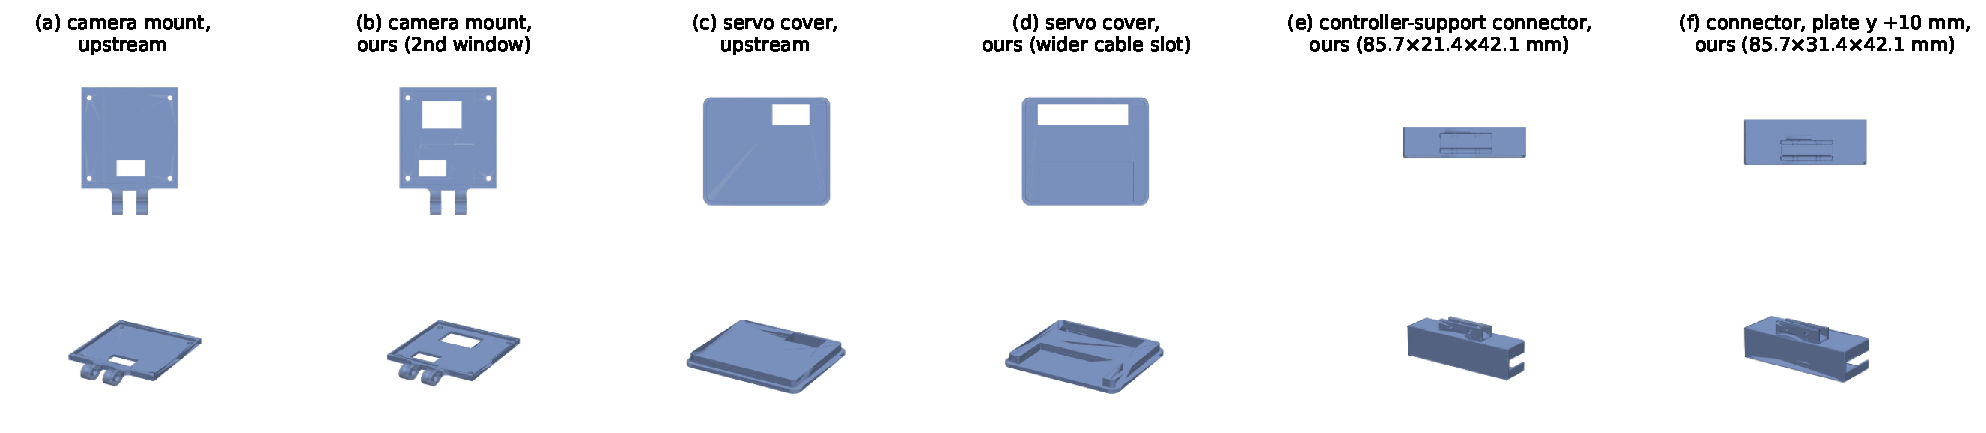
\includegraphics[width=\textwidth]{../figures/fig10_handumi_mods.pdf}
\caption{업스트림 HandUMI 부품에 대한 수정(출력 메시 렌더링). (a,b) 카메라 마운트: 기존 창 위에 두 번째 창 추가. (c,d) 서보 컨트롤러 커버:
케이블 구멍 확장. (e) 업스트림 VR 컨트롤러 지지대를 대신하는 새 왼손 컨트롤러 지지대 커넥터. (f) 그 클램프 플레이트를 10\mm 늘린 현재 버전.}
\label{p1:fig:hwmods}
\end{figure*}

\section{데이터셋 및 과제 설계}\label{p1:sec:data}
\textbf{기록.} 양손에 각각 HandUMI 장치를 착용한다(\ref{p1:sec:hw}절). 1920$\times$1080, 30\,fps 어안 카메라, 200\,Hz IMU, 100\,Hz로 샘플링하는
조 인코더로 구성된다. 머리에 고정한 Logitech C922가 탁자를 640$\times$480, 30\,fps로 기록하며, 이것이 정책에 주어지는 전역
시점이다(그림~\ref{p1:fig:dataset}a). 모든 스트림은 에피소드마다 MCAP 파일 하나와 영상 세 개로 저장된다.

\textbf{과제.} 50\mm 큐브 세 개(빨강, 파랑, 보라)를 고정된 접시 위에 여섯 순서 중 하나로 쌓는다. 지시문은 순서를 명시하며, 예를 들어
``Stack the blue cube on the bottom, purple cube in the middle, and red cube on the top, on the plate.''이다. 자동 루프가 음성
신호 후 20\,s 테이크를 기록하고, 조작자가 손으로 큐브를 다시 놓는 10\,s의 리셋 시간을 준다. 다음 순서는 가장 적게 수집된 순서(순서당
목표 50개)로 정해지므로, 순서는 무작위가 아니라 \emph{균형}을 맞춘 것이다. 큐브 배치는 수동 리셋을 통해 로봇 작업공간에 맞춘 기준
배치 주변에서 에피소드마다 달라지지만 기록되지 않았으며, 에피소드별 배치 레이블은 없다.

\textbf{수집.} 조작자 한 명이 사흘(2026년 9월 15--17일)에 걸쳐 15개 세션에서 에피소드 349개, 총 2.20\,h(에피소드 중앙값 23.05\,s)를
기록하였다. 순서별로 RBP 64, RPB 62, BRP 61, BPR 56, PRB 55, PBR 51이다(그림~\ref{p1:fig:dataset}b). 초기 10개 세션의 에피소드(55개)는
그리퍼 앵커를 사후에 도출했기 때문에 주 데이터 294개와 별도의 출처 도메인(``early'')으로 관리한다. 필터링 후 두 도메인은 비슷하게
동작한다.

\textbf{캘리브레이션.} 손목 카메라는 Kannala--Brandt 어안 모델을 사용한다(왼쪽 $f_x{=}789$, 오른쪽 $f_x{=}791$\,px). Kalibr 카메라--IMU
캘리브레이션 결과 시간 오프셋은 30.2, 32.8\,ms, 평균 재투영 오차는 6.0, 5.6\,px로 높은 편이며, 이것이 자세 정확도를 별도로 검증하는
이유 중 하나다(\ref{p1:sec:proc}절). 카메라--TCP 변환은 UMI가 CAD 상수를 쓰는 방식을 따라 캘리퍼로 측정한 값 $t=[0, 55.3, 122.5]$\mm{}와
고정된 축 치환을 사용한다. 이 값은 장치 하나에서 측정하여 양쪽에 적용하였다. 조 폭 스케일(개구 $67.5\pm5$\mm)은 50\mm 큐브 파지 영상으로
추정하였으며, 캘리퍼 확인은 아직 남아 있다.

\begin{figure*}[t]
\centering
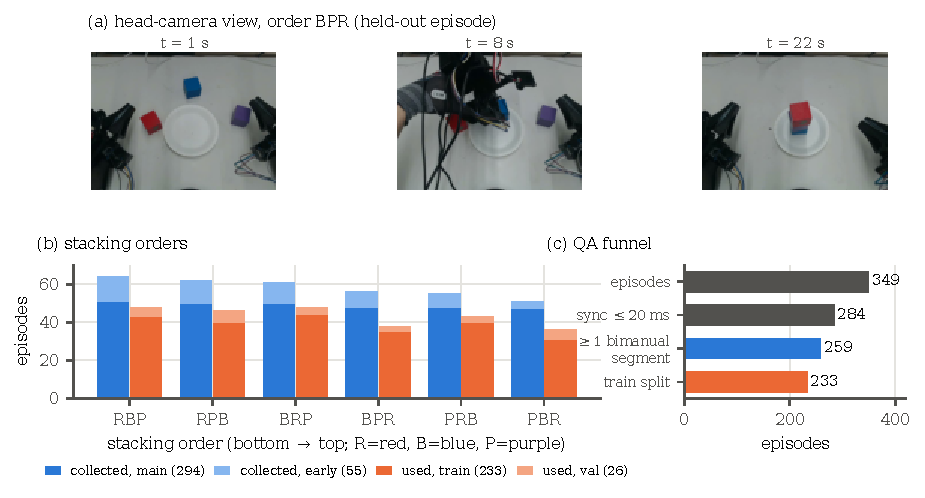
\includegraphics[width=\textwidth]{../figures/fig2_dataset.pdf}
\caption{데이터셋 설계. (a) held-out 에피소드(순서 BPR)의 1, 8, 22\,s 시점 헤드 카메라 프레임. (b) 쌓기 순서별 에피소드 수:
수집 시(main/early 도메인)와 처리 후(학습/검증). (c) 에피소드 수준 QA 퍼널.}
\label{p1:fig:dataset}
\end{figure*}

\section{처리 및 데이터 분할}\label{p1:sec:proc}
\textbf{손목 자세.} UMI는 모든 시연을 장면당 하나의 ORB-SLAM3 지도에서 위치 추정한다. 본 데이터에서는 이 방법이 실패하였다. 장면 변경
전에 만든 지도는 재위치 추정(relocalization)에 실패했고, 마커 벤치마크(아래)에서 그 궤적은 시연당 중앙값 3\%만을 덮었으며 위치 역전이
잦았다(역전율 중앙값 0.24, 채택한 방법은 0.07). 따라서 RGB 손목 영상만으로 MASt3R-SLAM을 실행하고, 에피소드마다 IMU로부터 메트릭
스케일을 복원한다(15프레임 윈도에 대한 시각--관성 피팅). ArUco 마커 에피소드 14개(손 궤적 28개, 그중 10개 held-out)로 이루어진 별도
벤치마크를 데이터셋과 같은 GPU에서 실행한 결과, 추적 커버리지 중앙값은 1.00(저장된 지도를 쓴 ORB-SLAM3는 0.03), 스케일 오차 p50/p90은
4.6/17.0\%(단일 전역 상수는 18.5/23.8\%), 회전 오차 p50/p90은 0.84/2.13\textdegree{}, UMI 방식 16스텝 상대 위치 오차 p90은 11.3\mm{}이다.
349개 에피소드 자체에는 정답(ground truth)이 없다.

\textbf{리타게팅.} 각 TCP 궤적은 URDF 기반 역기구학으로 reBot B601 6-DoF 팔에 매핑된다. 절대적인 작업공간 기하는 에피소드 간에 복원할
수 없으므로, 각 세그먼트를 고정된 로봇 시작 자세(로봇 원격조작 데이터의 활동 자세 중앙값)에 다시 앵커링한다. 즉 동작은 전이되지만 큐브의
절대 위치는 전이되지 않는다. 조 인코더 값은 이진 그리퍼 명령이 된다.

\textbf{게이트.} 표~\ref{p1:tab:funnel}에 퍼널을 정리하였다. 65개 에피소드가 65프레임 전체 윈도에 대한 $\le$20\,ms 동기화 요건을 통과하지
못한다. 나머지 284개에서 양팔 후보 세그먼트 1{,}306개가 나오며, 그중 677개는 로봇 작업공간을 벗어나고, 50개는 메트릭 스케일 검사에, 18개는
IK에 실패하여 561개(43.0\%)가 남는다. 두 세션(에피소드 6개)은 IMU--카메라 회전 불일치로 격리되었으며 세그먼트를 하나도 기여하지 않았다.
학습 단위는 65프레임(2.17\,s) 세그먼트이며, 세그먼트의 47\%가 에피소드 첫 5\,s 안에서 시작한다.

\textbf{분할.} 양팔 세그먼트가 하나 이상인 259개 에피소드를 에피소드 단위로 무작위 분할(seed 0, 10\%)하여 학습 233 / 검증 26, 즉
세그먼트 504/57개, 프레임 32{,}760/3{,}705개로 나눈다. 양쪽에 걸친 에피소드는 없다. 분할은 층화되지 않았으며, 검증 세트는 순서당 3--6
에피소드, main 22 / early 4개이고, 격리되지 않은 13개 세션 중 9개에서 왔다.

\begin{table}[t]
\centering\footnotesize
\caption{처리 퍼널(저장소의 집계 파일로부터 재계산한 수치).}
\label{p1:tab:funnel}
\setlength{\tabcolsep}{4pt}\begin{tabular}{@{}lrr@{}}
\toprule
단계 & 에피소드 & 세그먼트 \\
\midrule
기록됨(KEEP) & 349 & -- \\
자세 + 그리퍼 내보내기(궤적 698개) & 349 & -- \\
동기화 $\le$20\,ms, $\ge$65프레임 윈도 & 284 & 1{,}306 \\
\quad $-$ 작업공간 / 메트릭 스케일 / IK & & $-$677 / $-$50 / $-$18 \\
양팔 세그먼트 $\ge$1개(학습 풀) & 259 & 561 \\
\quad 학습 / 검증(에피소드 단위, seed 0) & 233 / 26 & 504 / 57 \\
\bottomrule
\end{tabular}
\end{table}

\section{모델 및 학습}\label{p1:sec:model}
공개 \texttt{xvla-base} 체크포인트에서 X-VLA~\cite{zheng2025xvla}(LeRobot 구현)를 파인튜닝한다. Florence-2 vision-language
인코더~\cite{xiao2024florence2}와 24층 트랜스포머 정책(hidden 1024, 헤드 16개, soft prompt 32개), flow matching 액션 헤드(디노이징
10스텝)로 구성되며, 파라미터 879M개가 모두 학습 대상이다. 입력은 세 시점(헤드, 왼손목, 오른손목; 224\,px로 리사이즈), 순서 지시문,
14-D 상태(팔마다 관절각 6개와 이진 그리퍼)이다.

\textbf{액션 목표.} 상태 시각 $t$에 대해 모델은 리타게팅된 의사 관절의 누적 관절 변위로 이루어진 30스텝 청크
$a_i = q_{t+5+i}-q_t$, $i=0,\dots,29$를 예측하며(5프레임 선행, 따라서 청크는 0.2--1.17\,s 앞을 덮는다), 여기에 절대 그리퍼 명령을
더한다. 두 보조 항이 관절 공간을 측정된 인간 동작에 묶는다. (C) 측정 궤적의 상대 TCP 위치를 남는 액션 차원에서 예측하는 항(가중치
2.0)과, (D) $\mathrm{FK}(q_t+\hat a_i)$와 측정 TCP 위치 사이의 순기구학 손실(가중치 20)이다. 목표는 측정된 인간 전이이며, 로봇
명령으로 다시 레이블링한 값은 절대 쓰지 않는다.

\textbf{최적화.} 300k 스텝, 배치 4, AdamW(lr $10^{-4}$, weight decay $10^{-4}$, warm-up 1k, $2.5\times10^{-6}$까지 cosine decay),
gradient clipping 10, fp32, RTX~4090 1대. 체크포인트는 10k 스텝마다 저장한다. 체크포인트 선택 규칙, 즉 전체 검증 샘플에 대한
최소 geo score(아래 참조)는 학습 전에 고정하였다.

\section{평가 프로토콜}\label{p1:sec:eval}
평가는 held-out 에피소드 26개에 대한 개루프 평가이다. 검증 세그먼트 57개 각각에서 시작 프레임 7개(0--30 구간에서 5프레임 간격)를
취해 샘플 399개, 팔-샘플 798개를 만들고, 예측 청크를 기록된 미래와 비교한다. 예측 구간 $k\in\{1,4,8,16,30\}$에 대해
$\mathrm{FK}(q_t+\hat a_k)$와 측정 TCP 사이의 TCP 위치 오차(중앙값, mm), 관절 MAE와 \emph{무동작} 예측기($\hat a\equiv0$)의 관절
MAE, 예측·측정 TCP 변위 사이의 코사인을 보고한다. \emph{geo score}는 다섯 예측 구간에 대한 TCP 오차 중앙값의 평균이다. 대부분의
샘플이 거의 정지 상태이므로, 모든 지표를 \emph{동작} 부분집합, 즉 $k{=}30$까지 측정 TCP가 $\ge$20\mm 움직이는 팔-샘플(798개 중
187개, 23.4\%)에 대해서도 보고한다. 이 게이트는 60k 체크포인트를 평가한 뒤에 추가되었으며 보고용으로만 쓴다.

\textbf{Prompt swap.} 지시문 사용 여부를 검증하기 위해 최종 체크포인트에 모든 샘플을 여섯 순서 지시문 각각으로 같은 노이즈 시드를
써서 질의하고, 올바른 지시문으로는 두 개의 추가 시드에서도 질의한다. 여섯 예측의 퍼짐은 지시문의 효과를, 시드 간 퍼짐은 샘플링
노이즈 하한을 나타낸다.

\textbf{분할이 검증하지 않는 것.} 검증 에피소드는 조작자, 장면, 세션, 여섯 순서 전부를 학습과 공유하며, 배치에는 레이블이 없다.
따라서 결과는 새 \emph{에피소드}에 대한 분포 내 일반화를 측정할 뿐, 새로운 배치·순서·장면에 대한 일반화를 측정하지 않는다.

\section{결과}\label{p1:sec:results}
\begin{table*}[t]
\centering\footnotesize
\setlength{\tabcolsep}{7pt}
\caption{오프라인 held-out 결과(에피소드 26개). TCP 오차: FK 위치 오차 중앙값(mm). MAE: 관절 MAE(deg), 괄호 안은 무동작 예측기.
cos: TCP 방향 코사인. 160k는 사전 등록된 선택, 300k는 최종 스텝이다.}
\label{p1:tab:results}
\begin{tabular}{@{}llccccc@{}}
\toprule
 & & \multicolumn{5}{c}{예측 구간 $k$ (5프레임 선행 후 1/30\,s 단위 스텝)} \\
\cmidrule(l){3-7}
부분집합 & 지표 & 1 & 4 & 8 & 16 & 30 \\
\midrule
\multirow{3}{*}{전체 (798)} & TCP 오차, 160k & 1.3 & 1.7 & 2.2 & 3.1 & 5.7 \\
 & TCP 오차, 300k & 1.5 & 1.8 & 2.2 & 3.2 & 5.7 \\
 & MAE, 300k & 0.30 (0.15) & 0.34 (0.19) & 0.42 (0.25) & 0.57 (0.36) & 0.97 (0.51) \\
\midrule
\multirow{4}{*}{동작 (187)} & TCP 오차, 160k & 11.2 & 15.0 & 19.9 & 29.2 & 39.1 \\
 & TCP 오차, 300k & 11.2 & 15.0 & 19.4 & 29.3 & 39.9 \\
 & MAE, 300k & 2.02 (2.32) & 2.68 (3.36) & 3.29 (4.38) & 4.30 (6.34) & 6.59 (8.68) \\
 & cos, 300k & 0.72 & 0.80 & 0.84 & 0.86 & 0.90 \\
\bottomrule
\end{tabular}
\end{table*}

표~\ref{p1:tab:results}와 그림~\ref{p1:fig:eval}에 평가 결과를 요약하였다. 네 가지 결과가 두드러진다.

\textbf{(1) 집계 오차는 주로 정지 구간을 반영한다.} geo score는 160k에서 2.78\mm, 300k에서 2.88\mm{}에 이르며 약 120k 이후로
평탄하다(그림~\ref{p1:fig:eval}a). 그러나 동작 샘플에서는 오차가 한 자릿수 더 크다. 가장 짧은 구간에서 11\mm, $k{=}30$에서 40\mm{}이며
p90은 90\mm{}이다. 동작 부분집합의 geo score는 23.0\mm{}로, 전체 샘플의 2.9\mm{}와 대비된다.

\textbf{(2) 동작 샘플에서 정책은 동작 방향을 예측하며 무동작 기준선을 앞선다.} 방향 코사인은 $k{=}1$의 0.72에서 $k{=}30$의 0.90으로
오르며, 관절 MAE는 모든 구간에서 무동작 예측기보다 13--32\% 낮다($k{=}30$에서 6.59 대 8.68\textdegree{}; 그림~\ref{p1:fig:eval}b).
모델은 다가올 동작의 존재뿐 아니라 그 방향도 포착한다.

\textbf{(3) 전체 샘플에서는 정책이 무동작 예측보다 나쁘다.} 관절 MAE는 모든 구간에서 무동작 MAE의 약 두 배이다($k{=}1$에서 0.30 대
0.15\textdegree{}). 정지 구간에서 정책은 작은 허위 동작을 예측하며, 예측 변위 대 측정 변위 비의 중앙값은 $k{=}1$에서 1.41이다.
$k{=}30$에서 예측의 퍼짐은 목표 퍼짐의 0.77배로, 긴 구간은 붕괴(collapse)되었다기보다 다소 과소 분산(under-dispersed)되어 있다.

\textbf{(4) 순서 지시문은 예측을 바꾸지만 개선하지는 않는다.} Prompt swap(그림~\ref{p1:fig:eval}c)에서 여섯 지시문은 동작 샘플의
$k{=}30$ 예측 TCP를 중앙값 4.8\mm{}만큼 움직이는데, 이는 샘플링 노이즈 퍼짐(0.09\mm)의 약 50$\times$이지만 예측 변위(62\mm)의 8\%에
불과하다. 올바른 지시문이 틀린 지시문보다 기록된 동작에 더 가깝지 않다. 올바른 지시문의 오차는 39.9\mm, 틀린 지시문 평균은 39.5\mm{}이고, 여섯 개
중 평균 순위는 3.55(우연 수준 3.5; 1위 비율 16\%, 우연 수준 17\%)이며, 모든 구간과 전체 샘플에서도 같은 양상이다. 올바른 지시문과 원래
시드로 얻은 예측은 기준 평가를 $10^{-5}$\mm 이내로 재현한다. 한 가지 단서는 2.2\,s 세그먼트의 상당 부분(뻗기, 들어 올리기)이 순서와
무관하다는 점이다. 선택 지점(에피소드의 첫 뻗기)으로 한정한 검증에는 검증 에피소드 26개가 제공하는 것보다 많은 샘플이 필요하다.

순서별 세부 결과는 저장소에 있다. 순서당 검증 에피소드가 3--6개뿐이어서 순서 간 순위를 매기기에는 너무 적으므로, 그 차이는 해석하지
않는다.

\begin{figure*}[t]
\centering
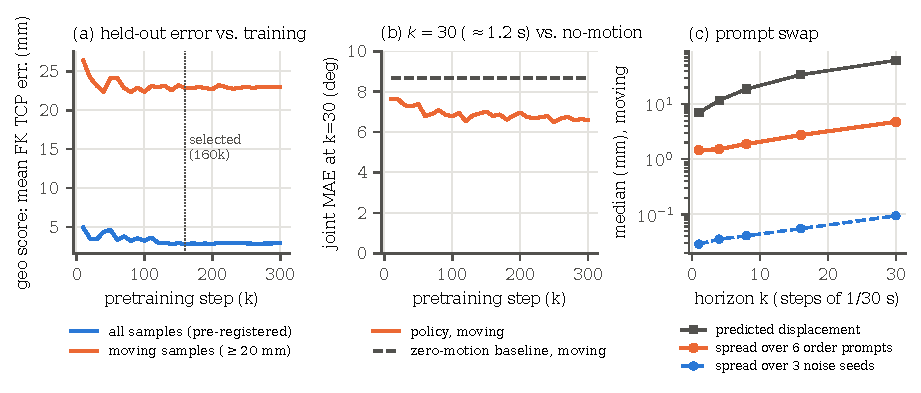
\includegraphics[width=\textwidth]{../figures/fig4_eval.pdf}
\caption{오프라인 평가. (a) 학습 과정에 따른 전체 대 동작 held-out 샘플의 geo score. 사전 등록 규칙은 160k를 선택한다.
(b) 동작 샘플의 $k{=}30$ 관절 MAE, 정책 대 무동작 예측기. (c) 최종 체크포인트에 대한 prompt swap: 여섯 순서 지시문(같은 시드)
간 예측 퍼짐 대 세 노이즈 시드(올바른 지시문) 간 퍼짐.}
\label{p1:fig:eval}
\end{figure*}

\section{실패 분석}\label{p1:sec:fail}
\textbf{과제 순서 지시문의 약한 사용.} 순서 프롬프트는 예측을 측정 가능한 수준으로 바꾸지만, 이 변화가 기록된 동작과의 일치도를
높이지는 않는다(결과 4). 이 데이터셋에서는 쌓기가 시작되면 순서가 장면에서 부분적으로 보이므로, 지시문은 에피소드 초반에만 필요하다.
학습의 어떤 요소도 모델이 지시문을 쓰도록 강제하지 않는다.

\textbf{정지 구간 드리프트.} 지배적인 오차 유형은 인간이 정지해 있는데도 0이 아닌 동작을 예측하는 것이다. 이것이 전체 샘플 MAE가
무동작 기준선보다 큰 이유이며, 로봇에서는 파지 전이나 놓은 후의 미세한 이동(creep)으로 나타날 것이다. 아직 검증하지 않은 그럴듯한
원인 하나는 거의 정지한 윈도에 남은 자세 노이즈로, 이것이 ``정지'' 목표를 노이즈가 많게 만든다.

\textbf{긴 구간의 과소 분산.} $k{=}30$의 예측은 목표보다 덜 변하고(비율 0.77), 동작 샘플의 p90 오차는 90\mm{}에 이르므로, 빠르거나
특이한 동작이 평균 쪽으로 끌려간다.

\textbf{학습 전 손실되는 데이터.} 후보 세그먼트의 57\%가 제거된다. 제거 745건 중 677건(91\%)이 작업공간 게이트에 의한 것이며, 그중
531건(78\%)에서는 한 팔만 로봇 작업공간을 벗어난다. 게이트가 동작의 범위로 동작을 제거하므로 남은 집합은 작은 동작 쪽으로 편향되었을
가능성이 높으나, 이 편향은 아직 정량화하지 않았다.

\textbf{설계를 결정지은 상류 단계 실패.} 저장된 지도를 쓴 ORB-SLAM3는 장면 변경 후 재위치 추정에 실패하고 위치 떨림을 만들었다.
이전 내보내기의 카메라 방향 규약 오류는 프레임 회귀 테스트로 발견되기 전까지 회전을 손상시켰다. 또한 65개 에피소드(19\%)가 동기화에
실패한다. 각각은 학습 손실이 아니라 명시적인 게이트로 발견되었다.

\section{후속 실험}\label{p1:sec:follow}
\textbf{리타게팅 v2.} \ref{p1:sec:proc}절의 단일 시작 앵커가 주된 손실 원인이었다. 모든 세그먼트가 하나의 로봇 자세에서 시작했기 때문에
대부분이 작업공간을 벗어났고, 리타게팅된 관절 궤적은 하나의 자세 클러스터만을 덮었다. 이를 엄격한 예산 아래의 다중 시드 리타게팅으로
대체하였다. 모든 실제 로봇 수치(시드 뱅크, 작업공간 게이트, 자세 페널티, 궤적 윈도)는 로봇 에피소드 30개에서만 가져오고, 결과는 이와
겹치지 않는 로봇 에피소드 120개에 대해 측정한다. 표~\ref{p1:tab:retarget}는 같은 후보 세그먼트 1{,}229개에서 네 변형을 비교한다. 각 인간
세그먼트를 가장 가까운 실현 가능한 로봇 궤적 윈도에서 시작하는 궤적 윈도 검색(TR)이 가장 로봇에 가깝다. held-out 로봇 데이터까지의 자세
거리가 1.49에서 0.27\,rad(중앙값)로 줄고, 시작 자세는 1개가 아닌 100개 클러스터에 걸친다. TR은 빠른 동작을 배치하지 못하므로 기구학
변형보다 해결하는 세그먼트가 적다. TR과 페널티를 둔 기구학 변형이 모두 해결하는 686개 세그먼트에서 두 방법의 관절 속도 분포는 비슷하므로
(W1 0.00207 대 0.00226), TR이 더하는 것은 동역학 개선이 아니라 자세 개선이다. 남은 실패는 거의 모두 ``작업공간과 호환되는 윈도
없음''이다(미해결 402개 중 399개).

\begin{table}[t]
\centering\footnotesize\setlength{\tabcolsep}{3.5pt}
\caption{259개 에피소드의 후보 세그먼트 1{,}229개에 대한 리타게팅 변형 비교, held-out 로봇 에피소드 120개 기준.
NN: 로봇 자세까지의 최근접 이웃 관절 공간 거리(rad, p50/p90). W1: 스텝당 $|\Delta q|$의 Wasserstein 거리.}
\label{p1:tab:retarget}
\resizebox{\columnwidth}{!}{%
\begin{tabular}{@{}lcccc@{}}
\toprule
변형 & 사용 가능 & NN p50 / p90 & 시작 클러스터 & W1 $|\Delta q|$ \\
\midrule
v1 단일 앵커 & 36.5\% & 1.49 / 1.55 & 1 & 0.00197 \\
v2-K 다중 시드 IK & 66.6\% & 1.21 / 1.60 & -- & 0.00275 \\
v2-Kr + 자세 페널티 & 67.0\% & 0.44 / 0.74 & -- & 0.00310 \\
v2-TR 윈도 검색 & 56.1\% & 0.27 / 0.45 & 100 & 0.00208 \\
\bottomrule
\end{tabular}}
\end{table}

\textbf{로봇 유사 재수집.} 손실이 수집 방식의 문제인지 검증하기 위해 수집기에 로봇 유사 프로토콜(30\,s 테이크, 로봇 통계와 비교한
실시간 손목 회전 속도 및 파지 피드백)을 추가하고, 한 세션에서 새 에피소드 60개(순서당 10개)를 기록하였다. 해석 규칙은 리타게팅 전에
고정하였다. 실시간 회전 속도는 절반으로 줄었으나(임계값 초과 비율 중앙값 0.144에서 0.067), 에피소드별 TR 수율은 변하지 않았고
(0.59 대 0.59) TR 사용 가능 비율은 56.1\%에서 58.9\%로 소폭 올랐을 뿐이다. 실시간 로봇 유사도와 TR 수율의 에피소드별 상관은 약하다
(Spearman $\rho=-0.11$, $p=0.05$, 통합 $n=316$). 실시간으로 측정한 로봇 유사 동작은 리타게팅 가능성과 연관되지만 그 대리 지표는
아니며, 작업공간 배치가 여전히 주된 실패 원인이다. 최종 TR 데이터셋은 두 수집분을 합친 것으로, 원본 에피소드 316개에서 나온 세그먼트
996개(학습 896 / 검증 100)이며 원래의 세그먼트 689개는 비트 단위로 동일하게 보존된다.

\textbf{로봇 파인튜닝을 위한 에고 사전학습.} 첫 릴리스 에고 체크포인트(\ref{p1:sec:model}절)와 base 체크포인트를 각각 같은 과제의 로봇
원격조작 에피소드 150개로, 같은 레시피·데이터·평가로 파인튜닝하였다. 초기값만 다르다. 맞춘 스텝 250k에서 에고 초기화 모델은 geo score가
10.0\% 낮고(에피소드 수준 paired bootstrap, 10k회 추출: 95\% CI $-14.7$에서 $-5.6\%$), 동작 샘플 geo score가 7.2\% 낮으며(CI $-13.4$에서
$-1.8\%$), $k{=}30$ 동작 관절 MAE가 6.8\% 낮다(CI $-12.7$에서 $+0.5\%$). 평가 에피소드 10개 중 8개가 에고 초기화 쪽에 유리하다. 평가
에피소드는 두 파인튜닝 세트 모두에 포함되어 있으므로, 이는 일반화가 아니라 각 모델이 로봇 학습 분포에 얼마나 잘 맞는지를 측정한다.
로봇 에피소드 90개로 한 더 작은 데이터 비교는 맞춘 스텝 두 개(10k, 20k)만 남기고 일찍 중단되었다. 여기서는 부호가 엇갈리므로(에고
초기화의 전체 샘플 geo $-33\%$와 $-11\%$, 동작 샘플 geo $+2\%$와 $+13\%$) 결론을 내리지 않는다.

\textbf{최종 데이터셋에서의 사전학습.} 996개 세그먼트 데이터셋으로 같은 레시피(계획 300k 스텝)를 써서 \texttt{xvla-base}에서 X-VLA를
사전학습하였다. 실행은 211.7k 스텝에서 중단되었고, 100k와 200k 체크포인트를 보관하며 100k를 이후 로봇 파인튜닝의 초기값으로 지정하였다.
이 체크포인트들로부터의 로봇 파인튜닝 결과는 여기서 보고하지 않는다. 위의 유일한 파인튜닝 비교는 첫 릴리스 에고 체크포인트를 사용한다.

\section{데카르트 에고 데이터(v3)}\label{p1:sec:v3}
로봇 관절로의 리타게팅(\ref{p1:sec:proc}절과 \ref{p1:sec:follow}절)에는 두 가지 비용이 있었다. 작업공간 및 IK 게이트가 후보 동작의 3분의 1에서
절반을 제거했고, 관절 공간 목표가 로봇 정책을 파인튜닝하는 데카르트 액션 공간과 달랐다. 버전 3는 의사 관절 단계를 없앤다. 각 인간 손목
궤적을 로봇 원격조작 데이터와 같은 상대 엔드이펙터 표현으로 직접 변환하여, 에고 샘플과 로봇 샘플이 하나의 텐서 계약을 공유하고 출처만
다르도록 한다.

\textbf{계약.} 행은 15\,Hz로 저장한다. 행 시각 $t$에 대한 액션은 미래 자세 16개의 청크 $A_k = T(t)^{-1}\,T(t + k\Delta)$, $k=1..16$이며,
$\Delta = 50.05$\,ms(로봇 데이터의 스텝, 합계 0.80\,s)이다. 이웃 행에서 가져오지 않고 원시 30\,Hz 궤적에서 보간한다(위치는 선형, 회전은
SLERP). 각 팔은 위치, 6-D 회전, 그리퍼 값을 제공하며(두 팔 합계 20차원, ``CART20''), 모델의 32-D 액션은 정확히 0이고 지도되지 않는 12개
차원으로 패딩된다. 상태는 각 팔의 자기 과제 시작 자세에 대한 상대 자세와 그리퍼 값 두 개로, 로봇 상태와 같은 배치이다. 그리퍼는 연속적인
조 개구를 80\mm{}로 나눈 값이며, 관측된 최댓값이 0.847이므로 ``완전 열림'' 끝에는 도달하지 않는다. 행은 $t$에서 두 팔이 모두 유효하고,
16개 목표 모두가 서로 50\,ms 이내 간격인 유효 원시 샘플 위에 있으며, 20\,ms 이내에 헤드 카메라 프레임이 있을 때만 남긴다. 패딩은 없다.
합성 테스트 11개가 계약을 고정한다. 그림~\ref{p1:fig:traj}는 레이블을 잘라내는 원천인 손목 궤적을 보여 주며, 전체 영상은 저장소에 있다.

\begin{figure*}[t]
\centering
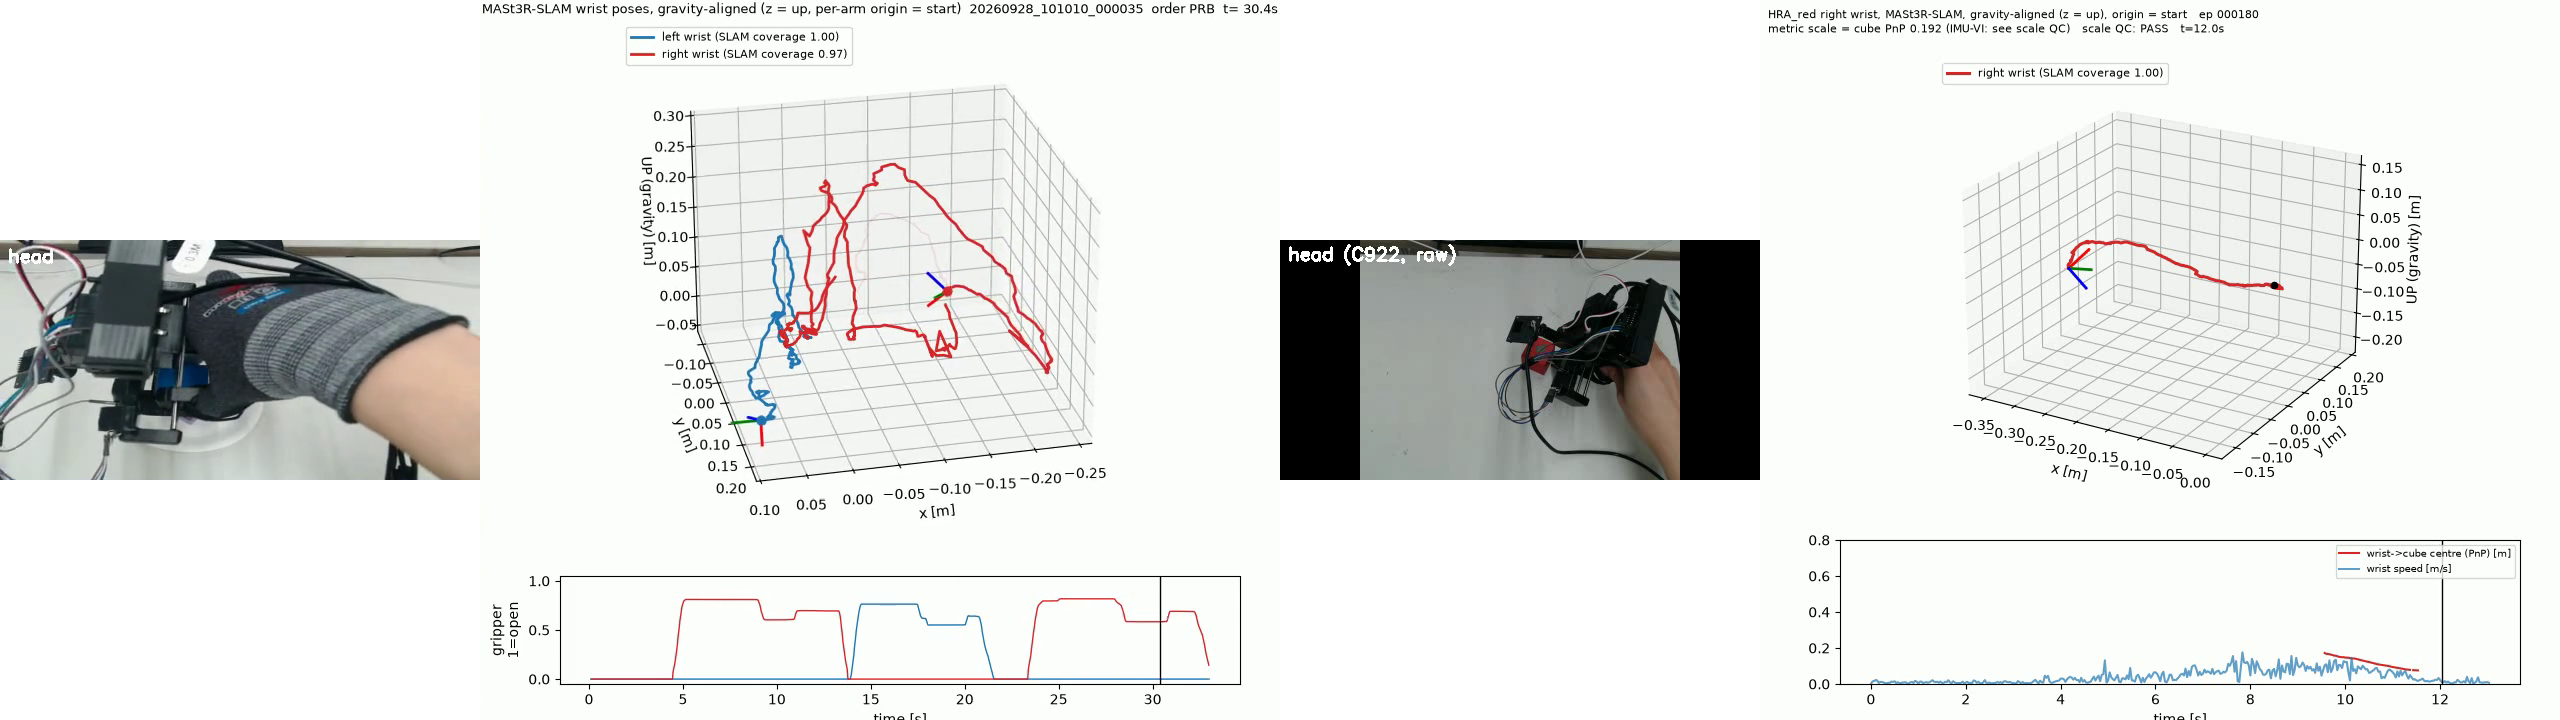
\includegraphics[width=0.8\textwidth]{../figures/fig7_mast3r_trajectories.png}
\caption{HRL80 쌓기 테이크(순서 PRB)의 MASt3R-SLAM 손목 궤적. 왼쪽: 헤드 카메라와 두 손목 어안 카메라. 오른쪽: 중력 정렬(z 위쪽)된
궤적으로, 각 팔의 원점은 시작 자세이고 현재 공구 축을 표시(x 빨강, y 초록, z 파랑)하며 메트릭 스케일은 IMU에서 얻었다. 아래: 두
그리퍼(1 = 열림). 세 테이크(PRB, RBP, PBR)의 영상은 저장소의
\texttt{docs/media/mast3r\_trajectories/hrl80\_0000\{35,55,60\}\_wrist.mp4}에 있다.}
\label{p1:fig:traj}
\end{figure*}

\textbf{데이터.} 원천은 손별 IMU 스케일이 유효한 원래 에피소드 273개와 HRL80 에피소드 60개이다. HRL80 에피소드 3개는 한 손의 IMU
스케일이 유효하지 않아 제외되어 330개가 남는다. 로봇 작업공간이나 IK 실현 가능성으로는 아무것도 필터링하지 않는다. 15\,Hz 행
111{,}533개 중 57{,}283개(51.4\%)가 학습에 사용 가능하며, 나머지는 추적 손실, 동기화 공백, 또는 에피소드의 마지막 0.8\,s에 걸린다.
분할은 이전 릴리스에서 고정한 것을 쓴다(검증 = \ref{p1:sec:proc}절의 held-out 에피소드 26개와 HRL80 에피소드 49--54). 학습 에피소드 298개에
행 51{,}612개, 검증 에피소드 32개에 행 5{,}671개이다.

\textbf{드러나지 않는 자세 점프.} 에고와 로봇의 상태 통계를 비교한 결과, 로봇 데이터에는 없는 행당 100\mm 초과의 상태 점프가 에고
데이터에 있었다. 두 원인이 섞여 있었다. 첫째, 내보낸 데이터셋에는 학습 행만 있으므로 ``인접'' 프레임이 수 초 떨어져 있을 수 있다.
30\mm{}를 넘는 겉보기 점프 2{,}598개 중 1{,}482개(57\%)가 이런 시간 공백이며, 인접 여부는 행 타임스탬프로 판단해야 한다. 둘째, 나머지
점프는 실제이다. MASt3R-SLAM은 추적 손실을 표시하지 않은 채 30\,Hz 한 프레임 안에서 카메라를 10\,cm 이상 옮기는 경우가 가끔 있다(학습
에피소드 24개에서 3\,m/s보다 빠른 원시 스텝 55개, 그 어느 것도 앞서 손실 플래그가 없었다). 상태는 과제 시작에 앵커링되어 있으므로 한
방향 점프는 그 에피소드의 이후 모든 상태를 손상시키는 반면, 현재 시점에 앵커링된 액션은 0.8\,s 동안만 영향을 받는다. v2b 필터는 한 방향
점프(행당 100\mm 또는 45\textdegree{} 초과, 또는 느린 두 스텝 사이의 고립된 50\mm 초과 스텝) 이후 에피소드의 나머지를 버리고, 고립된
스파이크는 그 스파이크만 버린다. 이 필터는 학습 에피소드 42개의 이벤트 44건에 작용하며 에피소드 하나를 통째로 제거한다. 학습은 에피소드
297개, 행 48{,}411개($-6.20$\%)로 줄고 검증은 변하지 않는다. 시간상 인접한 행 사이의 최대 스텝은 422.5에서 90.5\mm{}로, 100\mm 초과
스텝은 18개에서 0개로 줄며, 3\,m/s보다 빠른 원시 스텝 7개는 유효 행 안에 남는다.

\textbf{에고 데이터와 로봇 데이터의 차이.} 에고 에피소드 60개와 로봇 에피소드 60개에서, 에고 자세를 로봇 시작 자세에 붙였을 때 로봇
IK는 에고 위치의 99.7\%(왼쪽)와 99.5\%(오른쪽), 에고 전체 자세의 72.3\%/74.6\%에 도달한다. 로봇에서 쓰는 IK 구성은 손목 관절 하나를
잠그므로 로봇 \emph{자신의} 기록 자세도 45.2\%/52.2\%만 재현하는데, 이는 인간 데이터와 무관하게 존재하는 배포상의 한계이다. 에고 손은
더 작은 작업공간을 쓰고(상태 p95 0.221/0.214\,m 대 0.395/0.369\,m), 0.4\,s 이동량은 비슷하며(p95 93/99 대 91/100\mm), 에고는 두 손이
동시에 정지해 있는 경우가 훨씬 잦다(0.4\,s 기준 샘플의 19.5\% 대 2.4\%). 가장 큰 차이는 시각적이다. 선명도 척도인 이미지 Laplacian의
분산 중앙값이 에고 손목 어안 시점에서는 1{,}854/1{,}487, 로봇 손목 카메라에서는 59/64이다.

\section{전이 실험}\label{p1:sec:transfer}
이 절의 모든 실행은 하나의 레시피를 공유한다. 32-D 액션 헤드를 쓰는 X-VLA로, 손실은 액션 차원 0--19에만 걸고 차원 20--31은 입력과
출력에서 0으로 두며, 배치 8, 8-bit AdamW(정책 학습률 $10^{-4}$, warm-up 1k, 마지막 스텝에서 끝나는 cosine decay), bf16 혼합 정밀도,
seed 1000이다. 로봇 데이터는 같은 여섯 순서 쌓기 과제의 원격조작 에피소드 312개(프레임 174{,}012개)인 R312c이다. 파인튜닝은 새
옵티마이저로 시작하며 로봇 정규화 통계를 쓴다.

\textbf{어떤 soft prompt인가?} X-VLA는 soft prompt 집합을 선택하는 데이터셋/embodiment id를 조건으로 받는다. 이전 실행은 id~0을
썼다. 공개 base 가중치를 읽어 보면 슬롯 10--17만 학습되었다. 나머지 22개 슬롯에서는 인코더와 디코더 bias가 정확히 0이고 프롬프트
가중치가 초기값 근처에 머문다. 따라서 본 연구에서 쓴 id 0과 6은 모두 학습되지 않은 슬롯이었다. 학습된 슬롯이 더 나은 출발점인 것도
아니다. R312c에서의 초기 손실은 슬롯 0이 1.11, 6이 1.12, 15가 1.61, 10이 2.35, 16이 2.65, 17이 4.07, 11이 22.80이다. 아래의 모든 실행은
사용되지 않은 슬롯 20을 본 embodiment 전용 슬롯으로 쓴다.

\textbf{로봇 프레임에서의 에고 전용 모델.} 에고 데이터만으로 40k 스텝 학습한 뒤, 모델을 teacher forcing 방식으로 로봇 프레임 120개에
질의하고, 로봇 데이터로 40k 스텝 학습한 모델과 비교하였다(이 프레임들은 후자 모델의 학습 세트에 포함되므로 그 값은 상한 기준이다).
0.4\,s에서 예측 이동과 기록 이동 사이 코사인 중앙값은 로봇 모델이 $+0.81$/$+0.77$(왼쪽/오른쪽), 에고 모델이 $-0.05$/$-0.03$이다.
좌우 교환과 축 부호 반전의 어떤 조합도 에고 모델을 $+0.16$ 위로 올리지 못하며, 손목 카메라 광류(optical flow)는 두 도메인에서 TCP
동작과 같은 부호 관계를 가지므로, 이는 규약 오류가 아니다.

\begin{table}[t]
\centering\footnotesize\setlength{\tabcolsep}{3.2pt}
\caption{에고 전용 체크포인트(40k)에서 이미지와 상태가 서로 다른 도메인에서 올 때의 $k{=}4/8/16$ 방향 코사인 중앙값(왼쪽 $|$ 오른쪽).
에고 검증 프레임 100개와 로봇 프레임 100개, 셀당 동작 프레임 21--55개.}
\label{p1:tab:ablation}
\begin{tabular}{@{}lcc@{}}
\toprule
이미지 + 상태 & 왼쪽 $k$=4/8/16 & 오른쪽 $k$=4/8/16 \\
\midrule
에고 + 에고 & 0.87 / 0.91 / 0.92 & 0.89 / 0.94 / 0.84 \\
에고 + 0 & 0.77 / 0.80 / 0.89 & 0.85 / 0.80 / 0.66 \\
에고 + 로봇 & 0.76 / 0.81 / 0.90 & 0.72 / 0.69 / 0.72 \\
로봇 + 로봇 & 0.36 / 0.30 / $-$0.01 & 0.19 / 0.02 / $-$0.15 \\
로봇 + 0 & 0.17 / 0.25 / $-$0.25 & 0.24 / 0.06 / $-$0.02 \\
로봇 + 에고 & 0.16 / 0.24 / $-$0.16 & 0.49 / 0.33 / $-$0.03 \\
\bottomrule
\end{tabular}
\end{table}

\textbf{격차는 이미지에 있다.} 표~\ref{p1:tab:ablation}는 두 입력을 맞바꾼다. 에고 이미지를 주면 모델은 로봇 상태를 포함해 어떤 상태가
주어지든 0.69--0.90의 코사인을 유지하고, 로봇 이미지를 주면 상태와 관계없이 $-0.25$에서 $+0.49$ 사이로 떨어진다. 실패는 시각적이며,
이는 손목 시점의 30배 선명도 차이와 부합한다.

\textbf{초기값으로서의 에고 사전학습.} R312c에서 base 모델(A)과 50k 스텝 에고 모델(B)로부터 동일한 데이터, 스케줄(150k 스텝 cosine),
시드, 레시피로 파인튜닝하였다. 두 실행 모두 60k 근처에서 직접 중단하였다. 스텝 200에서 학습 손실은 A가 0.945, B가 0.244이다. 비율 B/A는
처음 5k 스텝에서 0.49, 5k--20k에서 0.875, 20k--40k에서 0.95이며, 55k--60k에서는 두 값이 동률이다(0.0733 대 0.0745, 기록된 24개 지점
중 13개에서 B가 낮음)(그림~\ref{p1:fig:egoinit}). 따라서 에고 사전학습은 로봇 데이터의 초기 피팅을 빠르게 하지만, 60k까지 학습 손실에서
측정 가능한 이점을 주지 않는다. 이는 조건당 시드 하나의 학습 손실이며, A와 B의 held-out 또는 폐루프 비교는 없다. 이후 300k 실행 두 개가
끝났으나 서로 다른 로봇 데이터셋(에고 초기화 실행은 R312c, scratch 실행은 에피소드 384개)을 썼으므로 전이 비교가 아니며, 전이 비교로
보고하지 않는다.

\begin{figure*}[t]
\centering
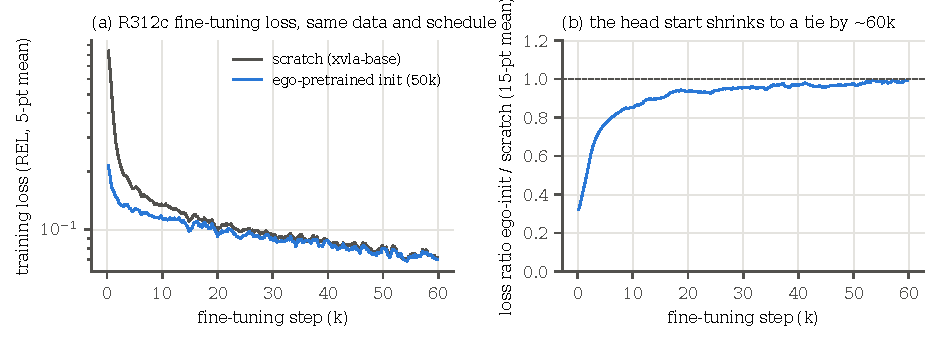
\includegraphics[width=\textwidth]{../figures/fig5_ego_init_loss.pdf}
\caption{같은 데이터·스케줄·시드에서 base 모델과 50k 에고 체크포인트로부터의 R312c 파인튜닝 비교. (a) 학습 손실. (b) 둘의 비율.
1 미만이면 에고 초기화에 유리하다. 학습 손실만 해당.}
\label{p1:fig:egoinit}
\end{figure*}

\textbf{시각적 격차를 줄이려는 시도.} 에고 손목 시점을 로봇처럼 보이게 하기 위해, 각 어안 프레임을 가상 핀홀 카메라(수평 화각
62--70\textdegree{}, 로봇처럼 조가 이미지 아래쪽에 오도록 주점을 이동)로 다시 렌더링한 뒤 다운샘플링, 블러, JPEG 압축을 적용한다.
레이블, 상태, 헤드 이미지는 바꾸지 않는다. 모든 프레임에 적용하면(ROBOT100) 손목 선명도 중앙값은 1{,}854/1{,}487에서 181/132로
떨어지지만, 여전히 로봇의 59/64보다 2--3배 높다. 프레임의 70\%를 다시 렌더링한 실행은 5k 스텝에서 중단하였고, 배치마다 정확히 에고
(ROBOT100) 샘플 4개와 로봇 샘플 4개를 쓰는 공동 학습 실행은 평가 없이 88.6k 스텝에서 중단하였다. 300k ROBOT100 사전학습 실행(에피소드
297개, 행 48{,}411개, 49.6 epoch)은 10월 5일 학습 손실 0.007로 끝났으며, 그 체크포인트들이 \ref{p1:sec:r30}절의 에고 초기값이다. 다시
렌더링한 모델에 대해서는 오프라인 전이 지표를 계산하지 않았다.

\textbf{로봇에서.} 위 모든 실행의 체크포인트를 배포 인터페이스를 통해 reBot에서 실행하였다. 10월 2일에서 4일 사이에 체크포인트 71개,
제어 사이클 49{,}431회, 실행 시작 1{,}681회이다. 사이클 로그는 과제 결과가 아니라 모델 자신의 웨이포인트에 대한 IK 추적을 기록하며,
에피소드나 지시문 필드가 없어 성공률을 산출할 수 없다. 조작자의 관찰 두 가지는 로그로 남지 않았다. 첫째, 파인튜닝 10k 스텝의 에고 초기화
모델은 큐브를 잡았으나 틀린 색을 집었다. 둘째, R312c로 300k 파인튜닝한 에고 초기화 모델(B300, 75k에서 205k 사이의 체크포인트)이
로봇에서 폐루프로 큐브 세 개를 끝까지 쌓았다. 시도 횟수는 기록되지 않았고 영상도 찍지 않았으므로, 폐루프 큐브 삼단 쌓기가 시연되었다는
사실만 말할 수 있으며 성공률은 없다. 이는 에고 사전학습의 가치에 대해서도 아무것도 말해 주지 않는다. 같은 R312c 데이터로 학습한
scratch 모델은 같은 프로토콜로 평가되지 않았다(완료된 scratch 300k 실행은 R384를 사용). 10월 5일에서 7일 사이 양팔 로봇 사용은 R384
scratch 모델(200k, 제어 사이클 4회)의 짧은 실행 한 번뿐이었다. \ref{p1:sec:lim}절에 나열한 필드를 갖춘 시도 로거가 10월 4일 배포
인터페이스에 추가되었으나 사용되지 않았으므로, 기록된 시도 결과는 여전히 없다. 10월 4일 저장소 정리에서 50k의 배수인 체크포인트만
남겼다. 큐브를 쌓은 B300 체크포인트 중 150k와 200k는 남아 있고 나머지(155k--205k)는 사라졌으므로, 시연은 150k 또는 200k에서만 재현할
수 있다.

\section{저데이터 Ablation: 로봇 에피소드 30개}\label{p1:sec:r30}
\ref{p1:sec:transfer}절의 312 에피소드 비교는 로봇 데이터가 초기값의 영향을 씻어 낼 여지를 충분히 준다. 인간 데이터 활용에 중요한 질문은
로봇 데이터가 부족할 때 도움이 되는지이다. 따라서 R312c의 에피소드 150--179인 R30(에피소드 30개, 프레임 17{,}600개, 쌓기 순서당 5개)으로,
\ref{p1:sec:transfer}절의 레시피, R312c 정규화 통계, seed 1000, 600k 스텝 cosine 스케줄을 써서 세 초기값에서 파인튜닝하였다. base 모델
(scratch)과, \ref{p1:sec:transfer}절의 ROBOT100 에고 사전학습 실행의 100k 및 300k 스텝이다. 100k 체크포인트는 같은 300k 스텝 스케줄의 중간에서
가져온 것이므로 학습률이 감쇠하지 않은 상태이며, 별도의 100k 스텝 실행이 아니다. 또한 두 에고 조건은 서로 다른 기계에서 실행되었으므로
(scratch와 100k-init은 RTX~4090, PyTorch~2.6; 300k-init은 RTX~5090, PyTorch~2.7.1) 비트 단위로 동일한 쌍둥이 실행이 아니다.

\begin{table}[t]
\centering\footnotesize\setlength{\tabcolsep}{4pt}
\caption{R30 파인튜닝, 맞춘 스텝에서의 학습 손실(200스텝 이동 평균)과 scratch 대비 윈도 평균의 비율(1 미만이면 에고 초기화에 유리).
조건당 시드 하나, held-out 또는 로봇 평가 없음.}
\label{p1:tab:r30}
\begin{tabular}{@{}lccc@{}}
\toprule
스텝 & Scratch & Ego-PT 100k 초기화 & Ego-PT 300k 초기화 \\
\midrule
200 & 0.801 & 0.239 & 0.446 \\
1k & 0.312 & 0.103 & 0.117 \\
10k & 0.065 & 0.056 & 0.040 \\
50k & 0.019 & 0.017 & 0.014 \\
100k & 0.009 & 0.009 & 0.007 \\
\midrule
윈도 & & 비율 & 비율 \\
\midrule
1k--5k & & 0.544 & 0.493 \\
10k--20k & & 0.823 & 0.697 \\
50k--100k & & 0.970 & 0.856 \\
100k--150k & & 1.021 & 0.914 \\
\bottomrule
\end{tabular}
\end{table}

\textbf{결과.} 표~\ref{p1:tab:r30}와 그림~\ref{p1:fig:r30}은 312 에피소드 비교와 같은 양상을 더 길게 늘여 보여 준다. 두 에고 초기화 모두 scratch
손실의 절반 미만에서 출발한다(1k--5k 윈도 비율 0.54와 0.49). 100k 스텝 초기화는 약 100k 스텝까지 이점을 잃고(50k--100k 비율 0.97,
100k--150k 비율 1.02), 300k 스텝 초기화는 더 작은 이점을 더 오래 유지하며(0.86과 0.91) 약 200k에서 동등해진다. 약 150k 이후로는 모든
손실이 출력 정밀도에서 0.001--0.004이므로 비율은 의미가 없다. 100k 스텝 초기화는 사전학습을 덜 했음에도 300k 스텝 초기화보다 낮게
출발하는데(스텝 200에서 0.239 대 0.446), 그 이유는 아직 설명하지 못했다. 세 실행 모두 GPU를 비우기 위해 471k(scratch), 305k(100k-init),
310k(300k-init)에서, 즉 214, 139, 141 epoch 후에 직접 중단하였다. 에피소드가 30개뿐이어서 모든 조건이 스케줄이 끝나기 훨씬 전에 학습
데이터에 거의 정확히 맞는다.

\textbf{이 결과가 보여 주는 것과 보여 주지 않는 것.} 30개 에피소드에서의 학습 손실은 각 초기값이 로봇 데이터를 얼마나 빨리 암기하는지를
측정할 뿐, 얼마나 잘 행동하는지를 측정하지 않는다. 모든 조건이 심하게 과적합하므로, 의미 있는 비교는 초기값 간 차이가 아직 남아 있는
초·중반 체크포인트(대략 10k--150k)에서의 폐루프 비교이다. 그러나 R30 체크포인트는 아직 로봇에서 실행되지 않았고 held-out 로봇 평가도
없다. 이 실험이 검증할 수 있는 예측은 에고 초기화 모델의 빠른 피팅이 더 적은 파인튜닝 스텝에서의 쌓기 성공으로 이어지는지이며, 이 실험은
아직 수행되지 않았다.

\begin{figure*}[t]
\centering
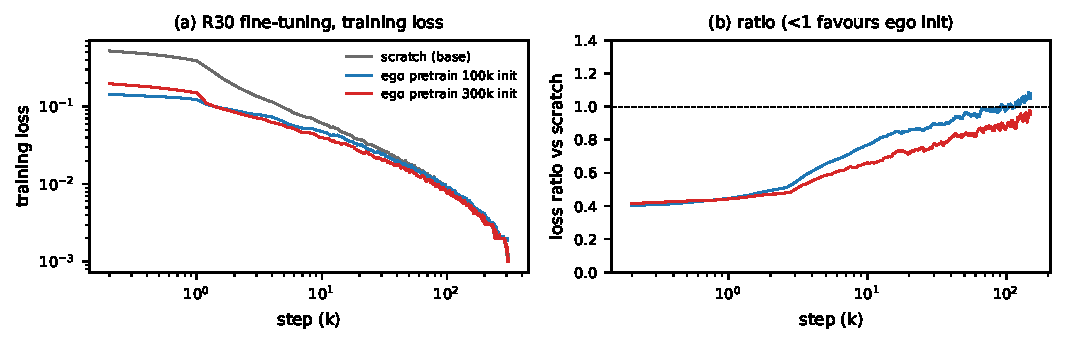
\includegraphics[width=0.8\textwidth]{../figures/fig8_r30_ablation.pdf}
\caption{base 모델과 100k·300k 스텝 에고 사전학습으로부터의 R30 파인튜닝(로봇 에피소드 30개). (a) 학습 손실(log--log, 평활화).
(b) scratch 대비 비율, 150k까지 표시. 그 이후는 소수점 셋째 자리 손실 때문에 비율이 노이즈가 된다. 학습 손실만 해당, 조건당 시드 하나.}
\label{p1:fig:r30}
\end{figure*}

\section{교훈}\label{p1:sec:lessons}
네 가지 발견이 작업 방식을 바꾸었으며, 각각은 손실 곡선이 아니라 명시적인 검사로 발견되었다. (i) 사전학습 모델의 조건화 인터페이스는
가정하지 말고 점검해야 한다. 본 연구의 embodiment id 두 개는 한 번도 학습된 적 없는 soft prompt를 가리키고 있었다. (ii) 인간 데이터와
로봇 데이터가 텐서 계약을 공유하면, 도메인 간 입력을 맞바꾸어 남은 격차의 위치를 찾을 수 있다. 여기서는 기구학이나 정규화가 아니라 손목
이미지였다. (iii) 모든 스케일 또는 자세 원천에는 드러나지 않게 실패하는 영역이 있다. 여기서는 드문 한 프레임 점프에서의 MASt3R-SLAM,
제2부에서는 느린 동작에서의 IMU 스케일이다. 두 경우 모두 독립적인 기준(로봇 통계, 알려진 물체)과 비교해서만 잡혔으며, 이제 이를 모든
새 수집에 포함한다. (iv) 초기값 간 학습 손실 비교는 로봇 데이터가 거의 0까지 피팅될 때마다 동률로 끝난다. 312개와 30개 에피소드 모두
그랬다. 이점은 초기 체크포인트에서의 held-out 또는 폐루프 평가로만 보일 수 있으며, 이를 위한 로깅은 로봇 실행 후가 아니라 그 전에
갖춰져 있어야 한다.

\section{한계 및 향후 연구}\label{p1:sec:lim}
\textbf{완료:} 데이터셋 수집과 캘리브레이션, 자세·리타게팅·QA 파이프라인, 300k 스텝 에고 파인튜닝과 held-out 에피소드 오프라인 평가,
리타게팅 v2, 로봇 유사 재수집, 150 에피소드 로봇 파인튜닝 맞춤 비교, 최종 996 세그먼트 데이터셋 사전학습(211.7k 스텝에서 중단,
체크포인트 100k와 200k). 버전 3에서 데카르트 에고 데이터셋과 필터, soft prompt 점검, 도메인 교환 진단, 60k 스텝까지의 초기값 맞춤 비교,
로봇 유사 손목 재렌더링을 추가하였다. 버전 4에서 완료된 ROBOT100 사전학습과 세 조건 R30 ablation(학습 손실, 305k--471k에서 중단)을
추가하였다. \textbf{조기 중단, 결론 없음:} 버전 2의 90, 60, 30 에피소드 로봇 파인튜닝 비교(맞춘 스텝 최대 두 개, 또는 한 조건만 실행),
70\% 재렌더링 사전학습(5k 스텝), 에고/로봇 공동 학습 실행(88.6k 스텝, 평가하지 않음).
\textbf{미수행:} 996 세그먼트 체크포인트로부터의 로봇 파인튜닝, R30 조건들의 로봇 또는 held-out 평가, 에고 초기화 모델과 scratch 모델의
held-out 또는 폐루프 비교, 로봇에서의 결과 로깅(로거는 있으나 기록된 시도가 없음). 버전 2의 로봇 평가 에피소드는 파인튜닝 데이터와
겹치므로, 겹치지 않는 로봇 데이터에서의 이점은 아직 보여야 한다.

\textbf{본 연구가 뒷받침하지 않는 것:} (i) 폐루프 성공률(로봇 에피소드 312개로 파인튜닝한 모델로 큐브 삼단 쌓기가 시연되었으나 시도
횟수를 세지 않음), 또는 에고 초기화 모델과 scratch 모델 간의 폐루프 차이, (ii) 새 큐브 배치로의 일반화(배치를 기록하지 않았고 설계상
절대 기하를 버림), (iii) 보지 못한 쌓기 순서로의 일반화(여섯 순서 모두 학습에 등장), (iv) 조작자 한 명, 장면 하나, 사흘을 넘어서는 전이,
(v) 로봇 학습 분포를 더 빨리 피팅하는 것 이상의 인간 데이터 이점, (vi) 에고 전용 정책 또는 재렌더링한 손목 이미지가 로봇 카메라로 전이된다는
것. \textbf{계획된 실험:} 모든 로봇 시도를 기록하고(모델, 체크포인트, 로봇 데이터 크기, 배치, 지시문, 쌓기 단계 0--3, 틀린 색, 실패 원인)
모델당 20--30회 시도한다. scratch 모델과 에고 초기화 모델을 맞춘 파인튜닝 스텝과 축소된 로봇 데이터(에피소드 30개)에서 비교하여 쌓기가
처음 성공하는 스텝 및 데이터 예산을 찾는다. 헤드 카메라로 배치를 기록하고 배치 영역을 held-out으로 둔다. 두 순서를 완전히 held-out으로
두고 지시문 추종을 검증한다. 정지 구간을 고려한 손실이나 가중치로 학습한다. 순서 지시문을 통제 변수로 하여 로봇에서 폐루프로 평가한다.

더 넓게 보면, 본 연구는 에고센트릭 인간 시연이 로봇 정책에 확장 가능한 지도 신호를 제공하는 연구 의제를 향한 첫걸음이다. 즉 embodiment
세부는 버리고 과제 기하와 의도는 유지하는 인간--로봇 표현을 학습하고, 실행 전에 예측 world model로 이를 평가하는 것이다. 현재 결과는
병목이 정책 못지않게 자세 복원, 필터링, 평가 설계에 있음을 보여 준다.

\section{결론}
큐브 삼단 쌓기의 양팔 에고센트릭 시연 349개를 수집하고, 게이트 기반 파이프라인으로 로봇 관절 공간 세그먼트 561개로 처리한 뒤, 그 결과로
0.9B VLA를 파인튜닝하였다. 오프라인에서 모델은 동작 샘플에 대해 held-out 인간 동작의 방향을 안정적으로 예측하고($k{=}30$에서 코사인
0.90) 무동작 기준선 대비 관절 공간 오차를 줄인다(구간에 따라 13--32\%). 정지 샘플에서는 허위 동작을 예측하며, 집계 지표는 이를 가리고,
순서 지시문을 바꾸어도 예측이 더 정확해지지 않는다. 다중 시드 궤적 검색은 리타게팅 손실의 상당 부분을 없애며, 에고 사전학습은 로봇
데이터로 파인튜닝할 때 작지만 일관된 이득을 주는데, 이는 로봇 학습 에피소드에서 측정한 것이다. 에피소드 전체를 로봇의 데카르트 액션 계약으로
변환하면, 드러나지 않는 SLAM 점프에 대한 필터를 거친 뒤 실현 가능성 필터 없이 에피소드 330개가 남는다. 이 계약 아래에서 남은 인간--로봇
격차는 시각적이다. 에고 전용 모델은 로봇 카메라 프레임에서 유용한 액션 방향을 주지 못하며, 격차는 상태가 아니라 손목 이미지를 따른다.
초기값으로서 에고 사전학습은 초기 로봇 파인튜닝을 빠르게 하고, 학습 손실상의 이점은 60k 스텝에서 사라진다. 로봇 에피소드 312개로
파인튜닝한 에고 초기화 모델이 로봇에서 큐브 세 개를 끝까지 쌓았으므로 과제 자체는 폐루프로 해결되었다. 에고 사전학습이 더 적은 로봇
에피소드나 더 적은 파인튜닝 스텝으로 그 지점에 도달하는지는 열린 질문이다. 느린 단일 팔 동작에서는 알려진 물체가 IMU 스케일을 대신한다.
공간 및 과제 순서 일반화, 겹치지 않는 로봇 데이터에서의 이점, 측정된 성공률에는 위에 나열한 통제 실험이 필요하다. 로봇 에피소드 30개에서도
에고 사전학습은 초기 피팅을 빠르게 하고, 사전학습이 길수록 더 오래 그러하며, 역시 학습 손실상의 이점은 사라진다. 그것이 초기
체크포인트에서 폐루프 이점이 되는지가 다음 실험이다.
\reportpart{제2부}{단일 팔 큐브 접근(Approach)}{part:p2}
\partabstract{제1부에서는 에고센트릭 인간 데이터와 로봇 데이터가 하나의 행동 계약(action contract)을 공유하면, 남는 격차가 기구학적인
것이 아니라 시각적·기하학적인 것임을 보였다. 제2부는 전이 가능한 가장 단순한 행동, 즉 에고센트릭 인간 시연만으로 학습한
오른팔의 빨간 큐브 접근을 따로 떼어 다룬다. 세 차례의 반복을 보고한다. (1) HRA\_red: 오른손 테이크 200개에서 IMU
시각-관성 스케일이 관측 불가능한 것으로 드러났다(중앙값 0.012, 95개 테이크에서 0 이하). 크기를 아는 3.8\,cm 큐브로부터
얻은 스케일이 이를 대체하며(IMU를 신뢰할 수 있는 양손 테이크에서 PnP/IMU 비 1.06), 166개 테이크가 남는다. 이 데이터로
학습한 0.9B X-VLA 모델은 첫 체크포인트부터 과적합한다(held-out 손실이 15k에서 0.150, 105k에서 0.299로 상승). 로봇에서는
가까운 시작점에서 큐브를 향해 움직였으나 먼 큐브에 대해서는 테이블 위를 끌며 이동했고, 로봇 보정(헤드 카메라, 0.16\,px
RMS의 손목 핸드-아이) 과정에서 FK TCP와 실제 조(jaw) 끝단 사이의 82\mm 오프셋을 비롯한 여러 규약 오류가 드러났다.
(2) 측정된 로봇 카메라 모델로 손목 영상을 재렌더링하고, 레이블을 핸드-아이 변환을 통해 로봇 TCP 자세로 표현하였다.
(3) HRA\_A100: 모든 테이크가 로봇도 터치한 테이프 원점 위에 그리퍼 끝을 대고 시작하는 새 프로토콜로, 공유 작업
좌표계(공선성 0.38\mm), 에피소드별 원점 yaw(오차 p50 0.21\textdegree), 테이블 평면으로부터의 두 번째 스케일 원천(큐브
PnP 대비 비 0.999)을 제공한다. 테이블 인지 변환은 107개 테이크 중 86개를 손끝 여유(clearance) 7.6\mm 이상으로 유지한다.
시작점 기준 상태와 원점 기준 상태는 같은 수준의 held-out 손실을 보이며(5k에서 0.124 대 0.132), 둘 다 5k부터 과적합한다.
로봇 실행에서는 근접 대리 지표로 큐브 크기 정지(cube-size stop)를 사용했으나(마지막 날 127개 세션 중 69개가 이로 종료),
시행 결과가 기록되지 않았으므로 성공률은 보고하지 않는다. 얻은 교훈의 대부분은 좌표계, 스케일, 배포 설정에 관한 것이며,
이를 우리가 해야 했던 수정 사항과 함께 정리한다.}
\section{서론}\label{p2:sec:intro}
눈에 보이는 물체를 향한 뻗기(reaching) 동작은 거의 모든 조작 작업의 첫 구간이며, 인간-로봇 전이~\cite{kareer2024egomimic}를
눈으로 판단할 수 있는 가장 단순한 동작이다. 팔이 큐브를 향해 움직이거나, 그렇지 않거나 둘 중 하나이기 때문이다.
제1부에서는 에고센트릭 데이터만으로 학습한 쌓기 모델이 로봇 카메라 프레임에서 유용한 행동 방향을 주지 못하며(코사인 중앙값
$-0.05$/$-0.03$), 이 격차가 손목 영상을 따라간다는 것을 확인했다. 단일 팔 접근 작업에서는 훨씬 적은 교란 요인으로 이
격차를 다룰 수 있다. 팔 하나, 물체 하나, 파지 없음, 작업 순서 없음이다. 제2부의 질문은 다음과 같다. \emph{에고센트릭
인간 시연만으로 학습한 오른팔 접근 사전(prior)이 로봇을 큐브 쪽으로 움직일 수 있는가, 그리고 그러려면 데이터가 어떤 조건을
만족해야 하는가?}

본 보고서의 기여는 다음과 같다. IMU에 의존하지 않는 느린 동작용 미터 스케일 원천(\ref{p2:sec:scale}절), 인간 데이터와 로봇
데이터를 하나의 작업 좌표계에 놓는 보정 체인(\ref{p2:sec:robotcal}절 및 \ref{p2:sec:a100}절), 학습 거동을 포함한 세 세대의
데이터셋(\ref{p2:sec:v1}--\ref{p2:sec:a100}절), 그리고 실제로 중요했던 배포 설정과 수정 사항(\ref{p2:sec:deploy}--\ref{p2:sec:corr}절)이다.
성공률은 보고하지 않는다. 이번 실행 동안 배포 인터페이스의 시행 기록기(trial logger)를 사용하지 않았기 때문이다.

\section{실험 구성}\label{p2:sec:setup}
\textbf{장치와 자세.} 작업자는 오른손에 HandUMI~\cite{handumi_hw} 한 대를 착용한다. HandUMI는 UMI 방식~\cite{chi2024umi}의 손 착용형
그리퍼(제1부 III절)로, 1080p30 어안 손목 카메라, 200\,Hz IMU, 조 엔코더로 구성된다. 고정된 Logitech C922가 테이블을
촬영한다. 손목 자세는 RGB 영상만을 입력으로 하는 MASt3R-SLAM~\cite{murai2025mast3rslam}에서 얻으며, 파이프라인은
제1부에 기술되어 있다.

\textbf{행동 계약.} 제1부의 20차원 데카르트 계약(CART20)을 그대로 사용한다. 행은 15\,Hz이며, 하나의 청크는 16개의 상대
자세 $T(t)^{-1}T(t+k\Delta)$($\Delta=50.05$\,ms)로 이루어지고, 팔마다 위치, 6-D 회전, 그리퍼를 담는다. 오른팔 전용
작업에서 왼팔은 더미(항등 자세, 그리퍼 0)이며, 그리퍼(조 미사용)와 함께 손실에서 마스킹되므로 20차원 중 9차원만
지도된다. 작업 문자열은 ``Approach to the red cube''이다.

\textbf{모델과 학습.} X-VLA~\cite{zheng2025xvla}(0.9B, LeRobot)를 제1부의 레시피로 학습한다. 소프트 프롬프트 슬롯 20,
배치 8, 8-bit AdamW(정책 학습률 $10^{-4}$), bf16, 시드 1000, 5k 스텝마다 체크포인트를 저장하며, RTX~4090에서 학습한다.
300 스텝 스모크 테스트로 loss mask를 검증했다. 마스킹·패딩된 차원은 정확히 0의 그래디언트를 받고, 지도되는 모든 차원은
0이 아닌 그래디언트를 받는다.

\textbf{로봇.} 손목 C922가 달린 reBot B601 오른팔을 Mac에서 pink IK 솔버로 구동한다. 로봇에서는 왼팔이 잠기고 양쪽 조가
고정되며, 배포 인터페이스는 이들에 대한 어떤 명령도 거부한다.

\section{HRA\_red: 물체 기반 스케일}\label{p2:sec:scale}
10월 3일 한 세션에서 ``빨간 큐브에 접근'' 오른손 테이크 200개(각 10\,s)를 녹화했다.

\textbf{느린 동작에서 IMU 스케일의 실패.} 쌓기 데이터에서는 잘 작동하던 에피소드별 시각-관성 스케일이 여기서는 관측
불가능하다. 접근 동작이 느리고 부드러워 가속도계가 스케일을 거의 구속하지 못하기 때문이다. 200개 테이크에서 IMU 스케일의
중앙값은 0.012이며, 그중 95개에서는 물리적으로 불가능한 0 또는 음수 값을 보인다(그림~\ref{p2:fig:cube}b).

\textbf{크기를 아는 큐브로부터의 스케일.} 빨간 큐브는 정지해 있으며 모서리 길이가 3.8\,cm이다. 큐브가 보이는 프레임에서
그 실루엣을 2면 또는 3면 모델로 피팅하고, 한 면이 정면에서 35\textdegree{} 이내로 보일 때는 단일 면 모델로 피팅한다. 이어
PnP를 풀고, 큐브가 움직이지 않는다는 조건으로부터 궤적 스케일을 닫힌 형태로 복원한다. 에피소드는 PnP 프레임 10개 이상,
부트스트랩 퍼짐 10\% 이하, 큐브 중심 잔차 2\,cm 이하일 때 유효하다. IMU 스케일을 신뢰할 수 있는 양손 HRL80 쌓기 테이크에서는
오른손 에피소드 57개 중 37개가 PnP 유효이며, PnP/IMU 비의 중앙값은 1.062(p16--p84 0.959--1.274; 그림~\ref{p2:fig:cube}a)이다.

\begin{figure*}[t]
\centering
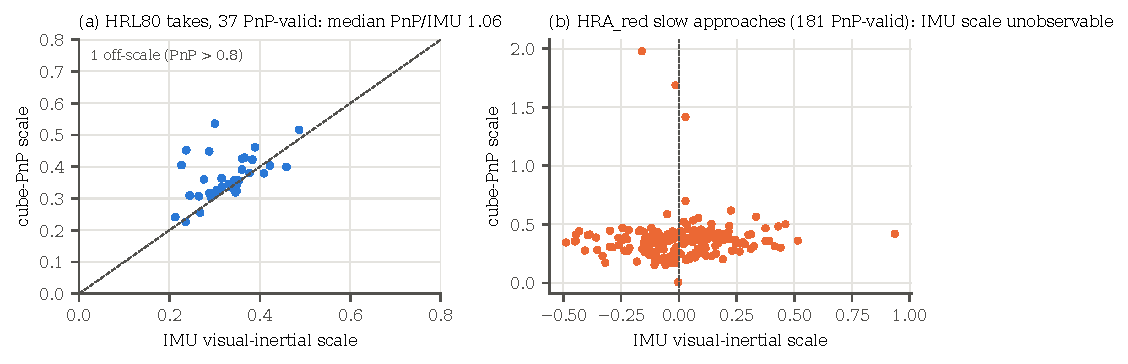
\includegraphics[width=\textwidth]{../figures/fig6_cube_scale.pdf}
\caption{IMU와 큐브 PnP로 구한 MASt3R-SLAM 궤적의 에피소드별 미터 스케일. (a) IMU 스케일을 신뢰할 수 있는 HRL80 쌓기
테이크. (b) HRA\_red 접근 테이크: IMU 스케일이 0 주변에 흩어진다.}
\label{p2:fig:cube}
\end{figure*}

\textbf{선별 과정.} 200개 테이크 중 19개가 스케일 게이트에서 탈락하고(PnP 프레임 부족 14개, 퍼짐 과다 5개), 15개가 스케일을
적용한 궤적의 물리적 타당성 검사에서 탈락한다(스케일 0.1--1.0, SLAM 이동 거리가 PnP로 관측한 접근 거리의 0.8배 이상, 이동
거리 0.8\,m 이하). 남은 166개는 학습 에피소드 151개(20{,}319행)와 검증 에피소드 15개(2{,}011행)로 나눈다. 스케일 중앙값은
0.354(p5 0.188, p95 0.500), 큐브 중심 잔차 중앙값은 0.17\,cm이다.

\section{HRA\_red v1: 학습과 첫 로봇 실행}\label{p2:sec:v1}
\textbf{학습.} v1에서는 제1부의 ROBOT100과 마찬가지로, 손목 어안 프레임을 \emph{추정한} 로봇 카메라(수평 화각
62--70\textdegree, 조가 영상 아래쪽에 오도록 주점을 이동)의 핀홀 뷰로 재렌더링했다. 300k 스텝 학습은 10월 5일 학습 손실
0.002(118 에폭)로 종료되었다. held-out 손실은 처음 평가한 체크포인트부터 상승한다(표~\ref{p2:tab:val}, 그림~\ref{p2:fig:val}a).
15k에서 0.150(학습 부분집합 0.066), 30k에서 0.198, 60k에서 0.213, 90k에서 0.265, 105k에서 0.299이며, 그동안 학습 부분집합
손실은 0.018까지 떨어진다. 에피소드 151개로는 모델이 거의 즉시 과적합한다. 15k 미만의 체크포인트는 평가하지 않았다.

\begin{table}[t]
\centering\footnotesize\setlength{\tabcolsep}{3pt}
\caption{체크포인트별 held-out 손실(지도되는 9차원에 대한 마스킹된 MSE). 괄호 안은 학습 부분집합 손실.}
\label{p2:tab:val}
\resizebox{\columnwidth}{!}{\begin{tabular}{@{}lccccc@{}}
\toprule
데이터셋(검증 에피소드) & 5k & 15k & 30k & 45k/50k & 105k \\
\midrule
HRA\_red v1 (15) & -- & 0.150 (0.066) & 0.198 (0.053) & -- & 0.299 (0.018) \\
A100 A: 시작점 (11) & 0.124 (0.110) & 0.125 (0.058) & 0.141 (0.031) & 0.224 (0.020) & -- \\
A100 B: 원점 (11) & 0.132 (0.097) & 0.147 (0.057) & 0.174 (0.031) & 0.190 (0.022) & -- \\
\bottomrule
\end{tabular}}
\end{table}

\textbf{첫 로봇 실행.} 10월 4일 15k--75k 체크포인트로 8{,}397 제어 사이클(실행 시작 658회)을 돌렸고, 10월 6일 오후에는
청크 실행 설정을 조정하면서(\ref{p2:sec:deploy}절) v1 100k, 200k, 300k로 계획 세션 61개를 실행했다. 작업자의 평가는
“정확도가 많이 떨어졌다”, “지그재그가 너무 심하다”였다. 큐브 가까이에서 시작하면 팔은 큐브를 향해 움직였고, 왼쪽으로 멀리
놓인 큐브에 대해서는 두 번의 실행에서 각각 약 39\,cm, 26\,cm 테이블 위를 끌며 이동했다. 이 실행들 중 결과가 기록된 것은
없다.

\section{로봇 측 보정}\label{p2:sec:robotcal}
이 실행들을 해석하려면 인간 데이터가 로봇에 대해 어디에 위치하는지 알아야 했지만, v1은 이를 전혀 다루지 않았다. v1의
레이블은 UMI 도구 좌표계의 상대 운동이고, 시작 상태는 인간 자신의 시작 자세이기 때문이다.

\textbf{헤드 카메라.} 고정 C922(HRA\_red 때와 같은 카메라, 같은 위치)를 25\mm 정사각형의 8$\times$5 체커보드로
보정했고(48프레임, RMS 1.05\,px, $f=728.7$\,px), 로봇 베이스에서의 카메라 자세는 TCP로 보드의 네 모서리를 터치하여
구했다(잔차 2--6\mm).

\textbf{인간 테이크와 베이스의 연결.} 각 테이크마다 헤드 카메라에서 큐브를 검출해 로봇 베이스에 배치하고, 손목 카메라의
큐브 PnP를 통해 손목 궤적을 여기에 연결한다. 기울기(tilt)는 테이블 법선에 대한 IMU 중력 방향에서, yaw는 큐브 면에서
얻는다. 이 방법으로 166개 테이크 중 64개를 연결했으며(병목은 헤드 카메라 검출), 내보낸 카메라--IMU 외부 파라미터에
18\textdegree{}의 회전 오류가 있음이 드러났다(수정 후 큐브 축 오차 17.8$\to$3.4\textdegree). 이전의 IMU 기반 기울기
통계는 최대 그만큼 틀려 있다. 학습 자세는 스케일을 큐브 PnP에서 얻으므로 영향을 받지 않았다. 이 연결은 이후 데이터셋을
구축하기에는 잡음이 너무 크다고 판단되었고(시작 높이가 4\,cm 범위로 퍼짐, 상방 축 오차 p50 10\textdegree, p90
28\textdegree), 이것이 \ref{p2:sec:a100}절 프로토콜의 동기가 되었다.

\textbf{로봇 손목 핸드-아이.} 보드 뷰 13장으로 0.16\,px RMS($f=651.4$\,px)의 손목 카메라 보정과, 네 가지 방법(Tsai--Lenz~\cite{tsai1989handeye}
포함)이 일치하는 핸드-아이 변환을 얻었다(베이스 내 보드 위치 퍼짐 1--2\mm, 0.3\textdegree). 카메라는 TCP보다 169.5\mm
뒤, 축에서 76\mm 벗어나 있으며, 광축은 TCP $x$축보다 33\textdegree{} 아래를 향한다. 테이크 시작 시점의 인간 손목 카메라와
도달 가능한 시작 자세에서의 로봇 손목 카메라는 일치시킬 수 없다. 인간의 시점을 맞추려면 어깨 관절이 한계를 넘어야 하기
때문이다. 가장 가까운 실현 가능한 시작 자세(자세 A)에서 카메라는 수평면 내에서는 1--14\mm 이내이지만, 78\mm 더 높고
8\textdegree{} 더 가파르다.

\textbf{TCP는 조 끝단이 아니다.} IK 스택의 TCP는 TCP $x$축을 따라 실제 조 끝단보다 약 82\mm 앞에 있다(FK 점을 손목
영상에 투영하여 확인). ``끝단이 테이블 아래로 내려간다''는 몇몇 판독은 이 인공물 때문이었으며 철회되었다. 이제 접촉 모델은
URDF 손끝 박스(TCP 뒤 70--80\mm, $\pm$19.6\mm)를 사용하며, 그 가장 낮은 모서리를 접촉으로 간주한다.

\textbf{v1 실행의 재해석.} 자세 A와 조 끝단 모델을 사용하여, v1 200k를 세 가지 규약으로 각각 한 번씩 실행한 결과는
다음과 같다. 도구 축을 회전하지 않으면 끝단은 큐브에서 약 2\,cm, 테이블 위 3\,cm에서 멈췄다. 카메라 피치 33.1\textdegree{}만큼
회전하면 약 11\,cm 지나쳤다. 회전과 함께 카메라--TCP 병진만큼 오프셋하면 큐브에서 약 4\,cm, 테이블 위 10\,cm에서 멈췄다.
이는 FK로 재구성한 단일 실행이며, 성공을 측정한 것이 아니다.

\section{로봇 카메라 렌더링(robotcam v2)}\label{p2:sec:v2}
v1은 추정한 카메라로 손목 뷰를 렌더링했다. 실측한 로봇 C922는 수평 화각이 52\textdegree{}이고 주점이 중앙에 있으므로, v1은
로봇 카메라보다 접근 과정에서 훨씬 늦게 큐브를 보여 주었다. v2에서는 모든 손목 프레임을 실측 내부 파라미터와 핸드-아이
자세로 렌더링하고, 레이블을 핸드-아이 변환을 통해 로봇 TCP 자세로 표현한다(로봇 TCP $\to$ UMI TCP: $y$축에 대해
$-33$\textdegree, $t=(-94.8, 2.4, 38.4)$\mm). 151/15 분할은 그대로이다. v2 학습은 약 64k 스텝(학습 손실 0.026)에서
중단되었다. v2와 초기 A100 테이크를 섞은 버전은 두 수집 데이터에 공통 원점이 없어 기각되었다(다음 절).

\section{HRA\_A100: 공유 원점}\label{p2:sec:a100}
\textbf{프로토콜.} 로봇 그리퍼에서 약 35\,cm 떨어진 헤드 카메라 베이스 플레이트 위의 테이프 십자 표시가 작업 원점이다.
각 테이크는 자동 사이클로 진행된다. 5\,s 휴식 후, 작업자가 HandUMI 조 끝단을 십자 위에 놓고 2\,s 동안 정지시킨다. 녹화는
녹화 구간 안에서 추가로 2\,s 홀드(원점)로 시작한다. 3\,s ``준비'' 단계에서 손을 로봇과 비슷한 시작 자세로 옮기고,
``시작(go)'' 신호에 10\,s 접근을 녹화하며, 학습 데이터는 ``go''부터 시작한다. 큐브 배치는 중앙 40, 좌/우 20, 앞/뒤 20,
가장자리 20으로 계획했다. 10월 6일 네 세션에서 107개 테이크를 확보했다(7, 8, 9, 83개. 첫 세션은 원점 홀드 도입 이전이다).

\begin{figure}[t]
\centering
\begin{tikzpicture}[font=\scriptsize, x=0.375cm]
\foreach \a/\b/\t/\c in {0/5/휴식/black!8, 5/7/정지/orange!20, 7/9/홀드/orange!45, 9/12/준비/blue!12, 12/22/접근(학습 데이터)/blue!30}
  {\fill[\c] (\a,0) rectangle (\b,0.55); \draw[black!50] (\a,0) rectangle (\b,0.55); \node at ({(\a+\b)/2},0.27) {\t};}
\foreach \x/\l in {0/0, 5/5, 7/7, 9/9, 12/12, 22/22\,s} \node[below] at (\x,0) {\l};
\end{tikzpicture}
\caption{HRA\_A100 테이크 사이클: 휴식, 테이프 십자 위에 조 끝단 정지, 2\,s 원점 홀드로 녹화 시작, 준비, 10\,s 접근.
원점 홀드는 HandUMI 조 끝단을 보정 시 로봇 조 끝단이 터치했던 것과 같은 테이프 십자 위에 놓는다.}
\label{p2:fig:protocol}
\end{figure}

\textbf{작업 좌표계 G.} 로봇 오른쪽 조 끝단으로 테이프 선 위의 세 점(먼 쪽, 중앙, 가까운 쪽)을 터치했다. 세 점은 60.4\mm
기준선에서 0.38\mm 이내로 공선이며, 높이는 2\mm 이내로 일치한다. G의 원점은 십자 중심이고, $x$축은 테이프를 따라 인간
쪽을 향하며, $z$축은 베이스 $z$축과 같다. 로봇 베이스에서 원점은 $(59.0, -74.9, 6.2)$\mm, 방위각은 47.09\textdegree{}이다.
35\mm 플레이트를 고려하면 테이블은 $z=-27.1$\mm{}에 있다.

\textbf{원점에서의 스케일과 방향.} 홀드 동안 손끝이 플레이트 위에 있으므로, 첫 MASt3R 키프레임의 포인트맵에는 카메라로부터
알려진 거리에 있는 테이블 평면이 포함된다. RANSAC으로 최대 세 개의 평면을 피팅하고(손가락 제외) 플레이트와 평행한 가장
큰 평면을 취하면 두 번째 스케일 원천이 된다. 40개 테이크에서 큐브 PnP 대비 비의 중앙값은 0.999, 에피소드별 오차는 p50 8\%,
p90 37\%이다. 각 에피소드는 큐브 PnP가 유효하면 이를, 그렇지 않으면 원점 평면을 사용하며(107개 중 각각 35개, 72개),
IMU는 사용하지 않는다. 원점 yaw는 십자 주변의 테이블을 매칭하여 에피소드마다 측정한다(오차 p50 0.21\textdegree, p90
1.17\textdegree). 평균 yaw를 가정했을 때는 잘못된 기각과 57\mm{}의 끝점 높이 퍼짐이 발생했다(측정 yaw 사용 시 35\mm).
홀드 자체의 반복성은 14\mm(p50; p90 37\mm), 6.2\textdegree(p50)이며, 이때 카메라는 63.7\textdegree{} 아래로 기울어져 있다.

\textbf{시작점 기준 대 원점 기준 상태.} 93개 테이크(학습 82, 검증 11. 제외된 14개는 이전 세션, 홀드 중 손이 20\mm 넘게
움직인 테이크 7개, 물리 검사 실패 1개)로, 다른 조건은 모두 같은 두 모델을 학습했다. A는 ``go'' 시점의 손 자세를 상태의
기준으로, B는 고정된 원점 좌표계 F(십자 위치, 테이프 방위, 홀드 피치 중앙값)를 기준으로 삼는다. 둘 다 로봇 TCP 레이블과
로봇 카메라 렌더링을 사용한다. 두 모델의 held-out 손실은 비슷하며 둘 다 첫 체크포인트에서 가장 낮다(표~\ref{p2:tab:val},
그림~\ref{p2:fig:val}b). 5k에서 A 0.124, B 0.132이고, 0.224(A, 50k), 0.190(B, 45k)까지 상승한다. 학습 테이크 82개로는 두
모델 모두 5k 스텝부터 과적합한다. 이 지표로는 어느 기준도 더 낫지 않다.

\begin{figure*}[t]
\centering
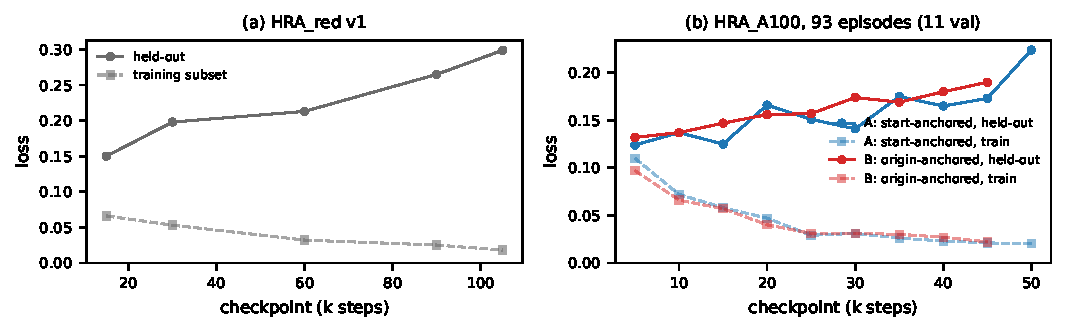
\includegraphics[width=0.8\textwidth]{../figures/fig9_hra_val.pdf}
\caption{체크포인트별 held-out 손실(실선)과 학습 부분집합 손실(점선). (a) HRA\_red v1, 검증 테이크 15개. (b) HRA\_A100,
시작점 기준(A) 및 원점 기준(B) 상태, 검증 테이크 11개. 모든 실행이 가장 이른 체크포인트부터 과적합한다.}
\label{p2:fig:val}
\end{figure*}

\textbf{테이블 인지 변환.} 인간의 동작을 G에서 표현하고 로봇 시작 자세에서 출발시키면 손끝이 테이블 속으로 들어갈 수 있다.
따라서 변환 과정은 테이크 동안 0으로 감쇠하는 가중치로 시작점을 로봇 시작 자세에 재고정하여 큐브 근처의 인간 끝점을
유지하고, 테이크마다 테이블+5\mm{}의 하드 하한과 12\mm{}의 선호 여유를 갖는 작은 이차 계획 문제를 푼다. 끝점은 최대 30\mm{}까지만
들어 올릴 수 있다. 표~\ref{p2:tab:ct}에 변형들을 정리했다. CT4는 위치, 높이, 회전을 각기 다른 스케줄로 감쇠한다. CT5는 측정된
원점 yaw, 보정된 IMU 중력, G에서의 절대 상태, 원점 홀드 게이트(홀드가 원점에서 10\mm 이내)를 추가한다. CT6는 로봇 시작
자세를 6\,cm 뒤, 4\,cm 아래로 옮긴다. CT5와 CT6는 손끝 여유 p50 12.6\mm, 최소 7.6\mm{}로 86개 테이크를 유지한다. 기각의
대부분은 이전 세션이거나 원점 yaw를 측정할 수 없었던 테이크이다.

\begin{table}[t]
\centering\footnotesize\setlength{\tabcolsep}{3pt}
\caption{HRA\_A100의 테이블 인지 변환. 채택 = PASS + PASS-CORRECTED. 여유: 보정 후 테이블 위 손끝 높이(채택된
테이크 기준).}
\label{p2:tab:ct}
\resizebox{\columnwidth}{!}{\begin{tabular}{@{}lcccc@{}}
\toprule
변형 & 테이크 & 채택 & 주요 기각 사유 & 여유 p50 / 최소 \\
\midrule
C (평균 yaw) & 107 & 81 & 들어올림 $>$30\,mm 10, 이전 세션 7 & 19.5 / 7.0\mm \\
CT4 (축별 감쇠) & 107 & 87 & 들어올림 10, 이전 세션 7 & 20.6 / 7.9\mm \\
CT5 (yaw, G, 홀드 게이트) & 107 & 86 & yaw 미측정 9, 이전 세션 7 & 12.6 / 7.6\mm \\
CT6 (시작점 뒤/아래) & 107 & 86 & CT5와 동일 & 12.6 / 7.6\mm \\
CT7 (낮은 시작점, +27) & 134 & 90 & IK 19, yaw 11, 이전 세션 7 & 12.4 / 7.6\mm \\
\bottomrule
\end{tabular}}
\end{table}

\textbf{시작 자세.} 로봇이 어디서 시작하는지는 시점과 도달 가능성 모두에 영향을 준다. G에서 인간 ``go'' 자세의 중앙값과
메도이드로부터 뒤, 오른쪽, 아래로 옮겨 도출한 시작 자세 후보 10개를 비교했다. 작업자는 가장 낮은 자세(자세 08, TCP
$(273, -168, 116)$\mm, 관절 여유 9.1\textdegree)를 선호했다. 10월 7일에는 더 낮은 인간 시작 자세로 27개 테이크를 추가
녹화했으나(원점에서 ``go''까지 약 247\mm 대신 약 89\mm), 자세 08 기준으로 5개만 통과하여 제외했다. 따라서 현재 학습
(CT7-old, 10월 6일 테이크 85개, 시작 자세 08, 100k 스텝 스케줄)은 10월 6일 데이터만 사용한다. CT5와 CT6 학습은 설정이
바뀌는 동안 각각 7k, 3k 스텝에서 중단되었으며, CT6와 CT7에는 검증 분할이 없다.

\section{중요했던 배포 설정}\label{p2:sec:deploy}
\textbf{청크 실행.} 인터페이스는 연속된 16스텝 청크를 블렌딩한다. 지수 블렌드 0.25, 크로스페이드 없음, 스무딩 없음,
청크당 최소 실행 행 1개일 때 동작은 수용할 만했다. 반면 코드 기본값(0.35, 4행, 3\textdegree, 6행)에서는 작업자가
“추론 품질이 많이 낮아졌다”고 보고했고, 이는 값을 복원할 때까지 지속되었다. 이 기본값은 10월 7일 인터페이스 재시작 시
조용히 되돌아가 있었다. 따라서 로봇에서의 추론 품질은 체크포인트에 포함되지 않는 설정에 좌우되며, 현재는 로더가 이
설정을 복원한다.

\textbf{도구 좌표계 규약.} 로봇 TCP 레이블로 학습한 모델(v2, A100)은 카메라 피치 0, 카메라--TCP 오프셋 0으로 실행해야 한다.
\ref{p2:sec:robotcal}절의 33.1\textdegree{} 피치와 오프셋은 v1에만 적용된다. 기준 고정(anchored) 모델은 같은 앵커 파일(B는
F, CT5--CT7은 G)로 서빙해야 한다.

\textbf{큐브 크기 정지.} 10월 7일 작업자는 팔이 멈추지 않고 큐브를 미는 것을 관찰했다. 이제 인터페이스는 0.1\,s마다 빨간
큐브의 겉보기 크기(원본 640$\times$480 손목 프레임에서 픽셀 단위 $\sqrt{\text{area}}$)를 측정하고, 두 번의 측정값이
임계값(170--250\,px 사용)을 넘으면 정지한다. 팔로우 모드(follow mode)에서는 큐브가 임계값의 85\% 미만으로 작아지면 재개한다.
큐브 크기 정지는 큐브가 손목 뷰에서 크게 보인다는 뜻일 뿐이며, 근접 대리 지표이지 검증된 접촉이 아니다. 또한 같은 위치에서
큐브가 학습 때보다 작게 보였기 때문에 손목 영상을 1.5$\times$ 확대했다.

\textbf{안전 장치.} v1 동안 인터페이스는 순 이동 450\mm, 추론 간 이동 80\mm, 정지 구간, 또는 250\mm{}나
60\textdegree{}를 넘는 출력이 발생하면 실행을 중단했다. 6\,s 시간 제한은 1--4 사이클 만에 실행을 끝내 버려 제거했다.
A100 모델에서는 모든 수치 안전 장치를 끄고, 왼팔과 조는 잠근 상태로 둔다.

\section{로봇 관찰}\label{p2:sec:robot}
인터페이스의 계획 실행 로그에는 10월 6일과 7일에 걸쳐 192개 세션이 기록되어 있다. 10월 6일의 65개 세션(v1 체크포인트,
앞서 기술한 청크 설정 조정)은 하나를 제외하고 모두 작업자가 중단했으며, 그 하나는 계획된 행이 90.9\textdegree{} 튀어
인터페이스가 종료했다. 10월 7일에는 127개 세션이 실행되었다. B 45k(3), A 50k(6), CT5 5k(4)에 이어 1.5$\times$ 확대를
적용한 B 50k(114개 세션, 다수가 팔로우 모드 재개)를 실행했다. 127개 중 69개는 큐브 크기 정지로, 58개는 작업자 중단으로
끝났다. 로그에는 결과 필드가 없고 시행 기록기를 사용하지 않았으므로, 몇 번의 접근이 큐브에 도달했는지 말할 수 없으며
성공률도 보고하지 않는다. 큐브는 어안 영상으로 렌더링한 학습 이미지에서는 주황색으로, 로봇 카메라에서는 빨간색으로 보이는데,
이 색 격차는 아직 보정하지 않았다.

\section{수정 사항}\label{p2:sec:corr}
우리 자신의 중간 판독 중 여러 개가 틀렸으며, 각각 독립적인 검사로 발견되었다. 로봇 시작 기울기는 3\textdegree{}가 아니라
25\textdegree{}였다. 로봇의 손목 뷰는 인간보다 2.5$\times$가 아니라 약 1.32$\times$ 확대되어 있고 11\textdegree{} 낮다.
``레이블이 끝단을 테이블 속 5\,cm까지 밀어 넣는다''는 판독은 TCP--끝단 오프셋 때문이었다. 테이블 높이는 접촉 모델을 고치면서
$-54.3$에서 $-5.9$, 다시 $-27.1$\mm{}로 바뀌었다. IMU 기울기 통계는 최대 18\textdegree{} 틀려 있었다. 평균 원점 yaw는 잘못된
기각을 일으켰다. 같은 오류는 어떤 인간-로봇 보정에서도 쉽게 저지를 수 있으므로 여기에 기록한다.

\section{교훈}\label{p2:sec:lessons}
(i) \emph{모든 스케일 원천에는 조용히 실패하는 영역이 있다}. 느린 동작에서의 IMU, 비스듬한 단일 면 뷰에서의 큐브 PnP,
일부 테이크에서의 원점 평면(p90 오차 37\%)이 그렇다. 실패를 알아차리려면 독립적인 두 번째 원천이 필요하다. (ii) \emph{공유된
물리적 원점은 사후 정합보다 저렴하다}. 166개 테이크를 사후에 헤드 카메라로 연결한 결과는 센티미터 단위 오차로 64개
테이크에 그쳤지만, 로봇과 인간이 모두 터치한 테이프 십자는 서브밀리미터 수준의 직선 피팅으로 공통 좌표계를 제공한다.
(iii) \emph{IK 스택의 TCP는 규약일 뿐 손끝이 아니다}. 접촉을 추론하려면 손끝 형상이 필요하다. (iv) \emph{작은 단일 작업
데이터셋은 즉시 과적합한다}. 80--150개 테이크에서는 held-out 손실이 첫 체크포인트(5k 또는 15k)에서 가장 낮으므로, 로봇에서
시험할 것은 이른 체크포인트이다. (v) \emph{실행 설정은 정책의 일부이다}. 인터페이스에 있는 블렌드·스무딩 파라미터가
체크포인트 교체보다 로봇 거동을 더 크게 바꾸었으므로, 모든 실행마다 함께 기록해야 한다.

\section{한계와 향후 과제}\label{p2:sec:lim}
성공률도, 로봇에서의 통제된 데이터셋 비교도 없다. 실행은 탐색적이었고, 실행 사이에 설정이 바뀌었으며, 결과는 기록되지
않았다. A100 데이터는 작업자 한 명, 장면 하나, 이틀에서 나왔고, held-out 집합은 11--15개 테이크이다. 큐브 색은 렌더링된
학습 이미지와 로봇 카메라 사이에서 다르다. 접근 데이터는 빨간 큐브 하나를 향한 방향을 가르칠 뿐이며, 색 그라운딩에
대해서는 아무것도 주장하지 않는다. 다음 단계는 다음과 같다. 실행 설정을 고정한 채 모든 로봇 시행(체크포인트, 시작 자세,
큐브 위치, 도달 여부, 정지 사유)을 기록한다. A, B, CT7의 이른 체크포인트(5k--15k)를 같은 시작 자세와 큐브 위치에서
시험한다. 선택한 시작 자세에서 A100 테이크를 더 수집한다. 렌더링된 손목 영상의 색을 보정한다. 그런 다음 접근 사전을
제1부 쌓기 정책의 첫 구간으로 사용한다.

\section{결론}
단일 팔 접근에서 에고센트릭 인간 데이터는 서브센티미터 수준의 일관성으로 로봇 좌표계에 들여올 수 있다. 다만 이는 IMU
스케일을 물체·평면 기반 스케일로 대체하고, 로봇 손목 카메라를 보정하며, 모든 테이크를 로봇과 공유하는 물리적 원점에
고정한 뒤에야 가능하다. 이러한 테이크 80--150개로 학습한 모델은 빠르게 과적합하며, 로봇에서는 가까운 시작점에서 큐브를
향해 움직인다. 결과가 기록되지 않았으므로, 얼마나 자주 큐브에 도달하는지는 여전히 열린 문제이다.
\reportpart{방법과 파이프라인}{각 단계의 작동 방식(제1부·제2부의 동반 문서)}{part:m}
\partabstract{본 문서는 에고센트릭 인간 시연을 로봇 정책으로 바꾸는 데 사용한 모든 단계를 알고리즘, 파라미터, 게이트 수준에서 기술한다. 손에
착용하는 기록 장치와 수집 프로토콜, 센서와 로봇의 캘리브레이션, 동기화와 내보내기, 단안 손목 자세 복원과 세 가지 메트릭 스케일
소스(IMU, 크기를 아는 큐브, 테이블 평면), 로봇 학습 데이터로의 두 세대 변환(관절 공간 리타게팅과 데카르트 액션 계약), 작업
프레임을 공유하는 단일 팔 변형, X-VLA 모델과 학습 레시피, 오프라인 평가와 진단 평가, 그리고 로봇 배포를 다룬다. 별도 언급이 없으면
파일 이름은 저장소 기준이다. 마지막 절에는 이 문서를 쓰는 동안 우리 코드에서 발견한 불일치를 나열한다.}
\section{개요}
그림~\ref{m:fig:overview}은 각 단계를 보여 준다. 각 단계는 출력을 매니페스트와 함께 기록하며, 그 뒤에 오는 게이트가 단위(에피소드,
세그먼트, 행 또는 테이크)를 승인하거나 사유와 함께 거부한다. 보고서는 각 게이트가 제거한 양을 센다. 두 변환은 앞단을 공유한다.
1세대(Gen-1)는 인간 손목 자세를 로봇 관절 궤적으로 리타게팅하고, 2세대(Gen-2)는 이를 우리 로봇 원격조작 데이터와 같은 상대
데카르트 액션 공간으로 표현한다. 단일 팔 접근 데이터(제2부)는 일부 차원을 마스킹하고 로봇과 물리적 원점을 공유하는 Gen-2 변형이다.

\begin{figure*}[t]
\centering
\begin{tikzpicture}[font=\scriptsize, node distance=3mm and 3mm,
  box/.style={draw=black!55, rounded corners=1.5pt, align=center, inner sep=2pt, minimum height=9mm, text width=24mm, fill=white},
  g1/.style={box, fill=orange!8, draw=orange!60!black}, g2/.style={box, fill=blue!7, draw=blue!55!black},
  dep/.style={box, fill=green!7, draw=green!45!black}, arr/.style={-{Stealth[length=1.5mm]}, draw=black!60}]
\node[box] (rig) {\textbf{장치 + 프로토콜}\\2$\times$HandUMI, 헤드 C922, AUTO 루프};
\node[box, right=of rig] (cal) {\textbf{캘리브레이션}\\어안, 카메라--IMU, 카메라$\to$TCP, 조, 로봇 카메라};
\node[box, right=of cal] (exp) {\textbf{내보내기 + 동기화}\\시계 피팅, $\le$20\,ms\\게이트, 그리퍼 폭};
\node[box, right=of exp] (pose) {\textbf{손목 자세}\\MASt3R-SLAM (RGB), 점프 필터};
\node[box, right=of pose] (scale) {\textbf{메트릭 스케일}\\IMU-VI $\mid$ 큐브 PnP $\mid$ 원점 평면};
\node[g1, below=6mm of rig] (g1) {\textbf{Gen-1}\\IK 리타게팅 $\to$ 의사 관절,\\65프레임 세그먼트};
\node[g2, right=of g1] (g2) {\textbf{Gen-2 CART20}\\상대 자세 16개, 15\,Hz 행, IK 필터 없음};
\node[g2, right=of g2] (hra) {\textbf{단일 팔}\\loss mask, G 프레임,\\테이블 인지 QP};
\node[box, right=of hra] (train) {\textbf{X-VLA 0.9B}\\사전학습 / 파인튜닝 /\\공동 학습 (Ray)};
\node[dep, right=of train] (dep) {\textbf{로봇}\\MPS 추론, Pink IK, PLAN 실행};
\draw[arr] (rig)--(cal); \draw[arr] (cal)--(exp); \draw[arr] (exp)--(pose); \draw[arr] (pose)--(scale);
\draw[arr] (scale.south) |- ++(0,-2.6mm) -| (g1.north); \draw[arr] (scale.south) |- ++(0,-2.6mm) -| (g2.north);
\draw[arr] (g2)--(hra); \draw[arr] (hra)--(train); \draw[arr] (train)--(dep);
\draw[arr] (g1.south) |- ++(0,-2.5mm) -| (train.south);
\end{tikzpicture}
\caption{파이프라인 개요. 주황: 1세대(관절 공간). 파랑: 2세대(데카르트)와 그 단일 팔 변형. 초록: 배포. 모든 화살표 뒤에는 사유를
기록하는 게이트가 있다.}
\label{m:fig:overview}
\end{figure*}

\section{기록 장치와 수집 프로토콜}\label{m:sec:rig}
\textbf{장치} (\code{collection/configs/handumi/hardware_handumi_v1.yaml}). HandUMI~\cite{handumi_hw}는 오픈소스 손 착용형 UMI 변형이다
(\url{https://github.com/murobotics-ai/handumi-hw}, 이전 \texttt{robonet-ai}). 커밋 \texttt{e58de33}의 본체, 링크, 서보 엔코더 조를 쓰고
VR 추적은 쓰지 않는다(제1부 III절). 각 HandUMI 유닛에는 Arducam 어안 UVC 카메라
(1920$\times$1080, 30\,fps, MJPG), Teensy~4.1에 연결된 ICM-42688-P IMU(공칭 200\,Hz, 보드마다 자체 오실레이터를 가지므로 실측은
201.6, 197.9\,Hz), 조(jaw) 인코더로 쓰는 Feetech STS3215 서보(4096 ticks/rev, 100\,Hz 폴링)가 달려 있다. 두 손목 카메라가 같은
USB 시리얼을 보고하므로 제품 이름으로 구분한다. 고정된 Logitech C922(640$\times$480, 30\,fps, 자동 초점 끔)가 탁자를 기록한다.
RGB-D 카메라는 손목 스트림을 방해하여 제외하였다.

\textbf{기록} (\code{collector/recorder.py}). 에피소드 디렉터리에는 카메라별 MP4 하나, \code{sensors.mcap}, \code{events.json},
\code{episode_meta.json}이 들어 있으며, 닫힐 때에만 이름이 \code{.incomplete}에서 \code{.complete}로 바뀐다. MCAP JSON 채널에는
IMU 샘플(장치·호스트 타임스탬프, 가속도계, 자이로), 그리퍼 샘플(언랩·랩 tick, 정규화 값), 프레임별 메타데이터(프레임 인덱스,
캡처 시각, 건너뛴 프레임), 이벤트, 시계 앵커가 담긴다. 모든 스트림에는 호스트 단조 시계로 타임스탬프를 찍는다. IMU는 호스트 수신
시각, 그리퍼는 시리얼 트랜잭션의 중간 시점, 프레임은 캡처 시각을 쓴다.

\textbf{AUTO 루프} (\code{collector/autoloop.py}). RESET $\to$ ARMING $\to$ HOLD $\to$ (PREP) $\to$ EPISODE $\to$ STOP 상태
기계가 음성 신호와 함께 각 테이크를 진행한다. ARMING은 정지 상태를 기다린다. 0.25\,s 창에서 자이로 크기의 평균이 6\textdegree/s
미만, 가속도 크기의 표준편차가 0.35\,m/s$^2$ 미만, 최대 샘플 간격이 25\,ms 미만, 창 채움률이 60\% 이상인 상태가 1\,s 동안 연속되어야
한다. 기록 시작 후의 정지 구간은 시각--관성 초기화 창 역할을 한다. 예비 QA를 통과한 테이크는 자동으로 보존되고, 실패하면 루프가
일시 정지한다.
\begin{itemize}
\item \emph{쌓기}: 20\,s 테이크, 10\,s 리셋, 3\,s 정지. 다음 순서는 보존된 테이크가 가장 적은 순서로 정해지므로
(\code{episode_manager.next_order}) 순서는 무작위가 아니라 균형을 맞춘 것이다.
\item \emph{로봇 유사}(\code{robot_like_v1}): 실시간 피드백이 있는 30\,s 테이크. 15\,Hz 격자에서 손목 각속도와 각가속도를 로봇
원격조작 데이터의 95번째 백분위수(0.996\,rad/s, 4.413\,rad/s$^2$)와 비교하며, 이를 넘는 틱이 10\% 초과이거나 파지가 두 번 미만이면
테이크를 검토로 보낸다.
\item \emph{접근}(HRA\_red): 오른손만, 10\,s 테이크, 5\,s 리셋, 그리퍼 검사 끔.
\item \emph{원점이 있는 접근}(HRA\_A100): 5\,s 휴식, 조 끝을 테이프로 표시한 십자에 대고 2\,s 정지, 2\,s 원점 정지를 추가로 하며
기록 시작(이벤트 \code{go_cue}), 로봇 유사 시작 자세로 3\,s ``ready'' 이동, ``go''에서 10\,s 접근. 오른 손목은 로봇 카메라와 비슷한
뷰도 기록한다.
\end{itemize}

\textbf{수집 QA} (\code{collector/integrity.py}). 장치나 레코더 오류 이벤트, 빈 스트림, 25\,fps 미만의 프레임률이 있으면 테이크를
검토로 보낸다. 그리퍼가 20\,Hz 미만으로 샘플링되거나, 멈춰 있거나, 캘리브레이션 범위를 300 tick 넘게 벗어나거나, 이동 거리가 범위의
5\% 미만이면 거부한다. 검증 단계에서는 모든 비디오를 디코딩하여 메타데이터 프레임 수와 맞는지 확인하고, 프레임 인덱스가 연속이며
캡처 시각이 엄격히 증가하는지 검사한다.

\section{캘리브레이션}\label{m:sec:cal}
\textbf{손목 카메라.} 전체 해상도에서 Kannala--Brandt(등거리) 어안 모델을 사용하며, 25\mm{} 정사각형의 8$\times$5 체커보드로
Kalibr로 피팅한다(왼쪽 $f_x{=}788.9$\,px). \textbf{카메라--IMU.} 손별 Kalibr~\cite{furgale2013kalibr} 외부 파라미터와 시간
오프셋. \textbf{카메라에서 TCP로} (\code{calibration/camera_tcp/handumi_camera_tcp_v2.yaml}). TCP는 집게 중심이며, $x$는 접근
방향, $y$는 조가 닫히는 방향, $z = x\times y$이다. 회전은 고정된 축 순열($x_\text{TCP}=z_\text{cam}$, $y_\text{TCP}=-x_\text{cam}$,
$z_\text{TCP}=-y_\text{cam}$)이고, 병진은 캘리퍼 측정값(앞으로 95\mm, 아래로 95\mm)을 IMU 중력으로 측정한 카메라 피치
(20.7\textdegree)만큼 회전한 것으로, $t=(0, 55.3, 122.5)$\mm{}를 얻으며 큐브 기반 피팅과 약 1\mm{} 이내로 일치한다. 이 값은
유닛 하나에서 측정하여 양쪽에 적용하였다. \textbf{헤드 카메라.} 임시 plumb-bob 모델($f=677.7$\,px).

\textbf{로봇 측}(제2부). 로봇의 고정 카메라는 같은 체커보드로 캘리브레이션한다($f=728.7$\,px, RMS 1.05\,px). 오른쪽 조 끝으로
내부 코너 네 개를 터치하고, 순기구학(FK) TCP 위치와 PnP로 구한 보드 자세를 Kabsch 정렬하여 $T_\text{base,board}$를 얻으며,
$T_\text{base,cam}=T_\text{base,board}T_\text{cam,board}^{-1}$이다. 로봇 손목 카메라는 보드 뷰 13장으로 캘리브레이션하고(종횡비
고정, 접선 왜곡 없음, RMS 0.16\,px), 핸드-아이 변환은 Tsai, Park, Horaud, Daniilidis 방법~\cite{tsai1989handeye}으로 풀어 Park의
해를 사용한다. 물리적 접촉은 URDF 손가락 끝 박스(IK TCP에서 $x$를 따라 뒤로 70--80\mm, $z$로 $\pm$19.6\mm)로 모델링하며, 그
가장 낮은 모서리를 접촉점으로 간주한다.

\section{내보내기와 동기화}\label{m:sec:export}
\textbf{시계 정렬} (\code{pose/timing.py}). USB 지연은 항상 지연을 더하기만 하므로, IMU 장치 시각을 최소제곱 기울기로 호스트 시각에
대응시키고 절편은 잔차의 5번째 백분위수에 다시 고정한다. 그다음 캘리브레이션에서 얻은 카메라--IMU 시간 오프셋을 적용한다. 카메라는
조금씩 다른 속도(30.003--30.026\,Hz)로 자유 동작하므로 프레임은 고정 오프셋이 아니라 가장 가까운 캡처 시각으로 짝짓는다.

\textbf{내보내기} (\code{pipeline/export/umi_export_orbslam.py}). 각 손목은 960$\times$540 비디오(내부 파라미터 절반), 첫 프레임
이전 50\,ms의 IMU를 포함한 GoPro 텔레메트리 형식의 IMU 파일, 카메라 설정 파일로 기록된다. 프레임과 캡처 시각은 단일 디코딩 패스에서
얻으므로 서로 어긋날 수 없다.

\textbf{동기화 게이트} (\code{pipeline/census/c8_census_pre.py}, \code{c8_phase3.py}). 왼 손목이 마스터 시계이고, 오른 손목과 헤드
카메라는 가장 가까운 캡처 시각으로 매칭한다. 두 손목 자세가 모두 유효하고 두 매칭이 모두 20\,ms 이내($\Delta t_R<20$\,ms,
$\Delta t_H<20$\,ms)이면 행이 유효하다. 연속된 유효 행 65개 이상의 구간이 하나라도 있으면 에피소드가 통과한다.

\textbf{그리퍼 폭} (\code{pipeline/grip/}). 각 프레임은 가장 가까운 그리퍼 샘플을 취한다. 기록된 정규화 값은 신뢰할 수 없었으므로
(열린 끝이 기계적 정지점 너머에 있었고, 왼쪽 방향이 세션마다 뒤집혔다) Gen-1은 raw tick으로부터 폭을 다시 계산한다. 방향은 열림/닫힘
tick 쌍에서, 닫힘 앵커는 에피소드별 닫힘 극값에서 정하고, 열린 끝은 닫힘 앵커에 장치 범위(1136.6 / 1248.2 ticks)를 더한 값이며,
폭 $= \mathrm{clip}(f,0,1)\times 67.5$\mm{}이다. Gen-2는 이후의 캘리퍼 캘리브레이션(gcal1)을 사용한다. 0/20/40/60/80\mm{}에 구간별
선형 보간점을 두고 $g=\mathrm{clip}(w/80\,\text{mm},0,1)$로 정규화하며, 0 = 닫힘이다.

\section{손목 자세와 메트릭 스케일}\label{m:sec:pose}
\textbf{단안 자세} (\code{pipeline/mast3r_pose/run_perframe.py}). MASt3R-SLAM~\cite{murai2025mast3rslam}(공식 코드, 커밋 고정,
유일한 패치는 빌드 수정)을 핀홀 뷰로 왜곡 보정한 RGB 손목 비디오에 대해 단일 스레드, 매 프레임, 고정 시드로 실행한다. 전역 최적화
후 모든 프레임을 최종 키프레임 기준으로 다시 표현한다.
\begin{equation}
T_{WC}(f) = T_{WK}^{\text{final}}(k)\,T_{WK}^{\text{track}}(k)^{-1}\,T_{WC}^{\text{track}}(f),
\end{equation}
이는 Sim(3) 사슬이다. 재위치추정(relocalisation) 중에 추적된 프레임은 이후 키프레임이 되지 않는 한 무효이다. 장면당 ORB-SLAM3 맵
하나를 쓰는 UMI 방식~\cite{chi2024umi}은 장면이 바뀐 뒤 재위치추정에 실패하여 대체하였다.

\textbf{IMU 시각--관성 스케일} (\code{cp6_scale.py:imu_vi}). SLAM 궤적은 에피소드별 스케일 $s$를 제외하면 메트릭이다.
$R_{wb}=R_{wc}R_{cb}$, 각 프레임 주위에서 박스 평균한 가속도계 샘플 $f_b$, 그리고 SLAM 카메라 위치와 $R_{wc}t_{cb}$의
Savitzky--Golay 2차 도함수(차수 3, 창 $W$)로 얻은 카메라 가속도 $a_\text{cam}$과 레버암 가속도 $a_\text{lever}$를 사용하면, 각
프레임은 다음 식의 세 행을 제공한다.
\begin{equation}
R_{wb}\,f_b - a_\text{lever} = s\,a_\text{cam} - g\;\;(+\,R_{wb}b_a),
\end{equation}
이를 가장 긴 유효 구간에 대해 Huber 가중 반복 재가중 최소제곱(10회 반복, $\sigma=1.4826\,$MAD)으로 $s$와 $g\in\mathbb{R}^3$에 대해
푼다. 양변이 같은 필터를 거치므로 대역 제한이 같고, 어떤 것도 두 번 적분하지 않는다. 바이어스 없는 $W=15$는 마커 벤치마크의 피팅
분할에서 선택하였다. $s>0$, $|g|\in[8.81,10.81]$\,m/s$^2$이고 $s$가 벤치마크 최소 스케일의 0.1$\times$와 최대 스케일의 10$\times$
사이에 있으면 스케일이 유효하다. 메트릭 TCP 자세는 $T_\text{tcp}=(T_{WC}\text{ with translation}\times s)\,X_\text{cam,tcp}$이다.

\textbf{자세 벤치마크.} 80\mm{} ArUco 마커 네 개가 보이는 시연 14개(손 트랙 28개, 피팅 9개, held-out 5개). 마커 자세는 왜곡 보정한
점에 대해 IPPE로 풀며, 합의 방향에서 20\textdegree{} 넘게 벗어난 마커는 버린다. 정답 스케일은 열 프레임 떨어진 프레임 쌍 중 마커가
30\mm{} 넘게 움직인 쌍에서 마커 변위와 SLAM 변위의 비의 중앙값이다. 커버리지, 스케일 오차, 회전 오차, UMI 방식의 16스텝 상대 위치
오차, 방향 반전 비율을 보고한다.

\textbf{카메라--IMU 일관성.} 자이로와 SLAM 각속도가 일치하지 않는 세션(다른 곳의 0.92--0.98 대비 코사인 중앙값이 0 근처)은 격리한다.
접근 데이터에서는 큐브 및 테이블 기하와 비교한 뒤, 오른 손목의 내보낸 카메라--IMU 회전을 카메라 $x$축에 대해 약
18\textdegree{} 수정하였다.

\textbf{자세 점프 필터} (\code{cart20/ego_cart20/preprocessing/pose_filter.py}). MASt3R-SLAM은 가끔 손실 플래그 없이 한 프레임 안에
카메라를 수 센티미터 움직인다. 한 66.7\,ms 행 동안의 변위가 100\mm{} 또는 45\textdegree{}를 넘고 점프가 그 스텝 안에 있을 때, 또는
50\mm{}를 넘는 스텝이 0.3\,m/s보다 느린 스텝들 사이에 고립되어 있을 때 raw 스텝에 플래그를 단다. 5샘플 이내의 플래그는 하나의
이벤트로 묶는다. 자세가 되돌아오면($\max(30\,\text{mm}, 0.3\times\text{step})$와 45\textdegree{} 이내) 이벤트는 스파이크이며 해당
샘플만 무효화한다. 그렇지 않으면 단방향 점프로 보고 그 팔 트랙의 나머지를 무효화한다. 시작점에 고정된 상태가 그 이후로 틀리게 되기
때문이다.

\textbf{큐브 PnP 스케일} (\code{cart20/ego_cart20/cube_pnp.py}, 제2부). 느린 동작에서는 IMU 피팅이 관측 불가능하다. 빨간 큐브(모서리
38\mm)를 HSV로 분할하고, 볼록 껍질을 꼭짓점 여섯 개(또는 네 개)로 줄인 뒤 각 변의 가운데 부분에 대한 직선 피팅으로 모서리를
날카롭게 다듬는다. 이를 2면·3면 실루엣 모델로 PnP 피팅하거나(가시성 검사: 카메라가 앞쪽에 놓이는 면들이 모델의 보이는 면과 같아야
한다), 정면에서 35\textdegree{} 이내이면 중심을 면 뒤쪽 반 모서리 거리에 둔 단일 면 IPPE 모델로 피팅한다. 큐브가 정지해 있으므로 그
중심 $c_i=p_i + k\,R_i t_i$는 일정해야 하며, 이로부터 역스케일을 닫힌 형태로 얻는다.
\begin{equation}
k = -\frac{\sum_i (p_i-\bar p)\cdot(u_i-\bar u)}{\sum_i\lVert u_i-\bar u\rVert^2},\qquad u_i=R_i t_i,\quad s=1/k,
\end{equation}
여기에 MAD 트리밍과 부트스트랩 재표본 200회를 적용한다. 테이크는 PnP 프레임 10개 이상, 부트스트랩 퍼짐 10\% 이하, 중심 잔차
2\,cm 이하를 만족해야 한다.

\textbf{원점 평면 스케일}(제2부, HRA\_A100). 원점 정지 동안 손가락 끝이 판에 닿아 있으므로 첫 SLAM 키프레임은 알려진 거리에서
테이블을 본다. 손가락 영역과 신뢰도가 낮은 점을 제외하고 RANSAC(400회 반복, 임계값은 깊이 중앙값의 0.4\%)으로 평면을 최대 세 개
피팅하며, 첫 평면과 평행한 것 중 가장 큰 평면을 테이블로 택한다. 그러면 $s=|n\cdot t_\text{tip}|/(s_0\,|d|)$이며, $t_\text{tip}$은
카메라 좌표계의 손가락 끝, $s_0$는 키프레임의 Sim(3) 스케일이다. 큐브 PnP가 유효하면 그것을, 아니면 평면을 사용한다.

\section{1세대: 관절 공간 리타게팅}\label{m:sec:gen1}
\textbf{세그먼트와 게이트} (\code{c8_phase3.py}). 유효 행을 겹치지 않는 65프레임 블록(2.17\,s)으로 자른다. 팔별로 세그먼트는 유효한
메트릭 스케일을 가져야 하고(B), 행의 95\% 이상이 로봇 작업 공간 안에 있어야 하며(C; 목표는 로봇 원격조작 TCP 자세 6{,}000개 중
최근접 이웃이 50\mm{} 이내이고 가장 가까운 50개의 방향 차이 중 최솟값이 20\textdegree{} 미만이면 내부로 본다), 모든 행에서 IK가
풀려야 하고(D), 유한한 관절 값을 내야 한다(E). 두 팔이 모두 통과하면 세그먼트는 양팔 세그먼트이다.

\textbf{리타게팅} (\code{pipeline/pseudo_joint/pseudo_joint_pipeline.py}). 인간 동작을 세그먼트 시작 기준 상대 동작으로 취해 로봇
데이터셋의 TCP 프레임으로 옮기고($\text{rel}=F^{-1}T_{0}^{-1}T_{t}F$, $F=R_x(180^\circ)$), 고정된 로봇 앵커 자세(로봇 원격조작
데이터의 활동 자세 중앙값)에 배치한다. $T_\text{tgt}=\mathrm{FK}(q_\text{anchor})\,C^{-1}\,\text{rel}\,C$, $C=R_y(90^\circ)$.
최소제곱 IK(방향 가중치 20의 자세 비용, 이전 해를 향한 rest 항, 관절 한계 제약, 최대 10회 반복, 관절 스텝 최대 0.35\,rad)는 이전
행에서 시드를 받는다. 행에는 LIMIT, DQ\_FAIL($>$1\,rad), BRANCH\_SWITCH(목표가 거의 움직이지 않는데 $>$0.3\,rad), NOT\_CONVERGED
($>$15\mm{} 또는 $>$5\textdegree), OK 중 하나의 레이블을 붙인다.

\textbf{데이터셋과 목표} (\code{pipeline/dataset/}, \code{training/humanik_delta.py}). 세그먼트당 LeRobot 에피소드 하나이며,
640$\times$480 뷰 세 개, 14차원 상태(팔마다 관절 각도 여섯 개와 그리퍼 값 하나), 목표 TCP 자세로 구성된다. 정책은 누적 관절 변위
30개 $a_i=q_{t+5+i}-q_t$(5프레임 선행)와 절대 이진 그리퍼를 예측한다. 두 보조 손실이 관절 공간을 측정된 동작에 묶는다. (C) 여분
액션 차원에 상대 TCP 병진 $\mathrm{trans}(T_\text{tgt}(t)^{-1}T_\text{tgt}(t{+}5{+}i))\times10$을 두는 항과, (D) FK 일관성 항이다.
\begin{equation}
\mathcal{L}=\mathcal{L}_{\Delta q}+\mathcal{L}_\text{grip}+2.0\,\mathcal{L}_C+20\,\lVert \mathrm{FK}(q_t+\hat a)-p_\text{tgt}\rVert^2 .
\end{equation}
분할은 고정 시드로 원본 에피소드의 10\%를 뽑으며, 양쪽에 걸치는 에피소드는 없다.

\textbf{리타게팅 v2} (\code{pipeline/retarget_v2/}). 단일 앵커 때문에 모든 세그먼트가 한 자세에서 시작했다. v2는 캘리브레이션에 로봇
에피소드 30개만 사용한다(다른 120개로 평가). 두 팔 관절의 $2^{17}$개 Sobol 샘플로 된 시드 뱅크를 작업 공간, 테이블 바닥, 조작성
(위치 야코비안의 최소 특이값), 팔 간 간격 $\ge$75\mm{}(팔당 링크 세그먼트 9개 사이의 정확한 세그먼트 간 거리)로 거른 뒤 중복을
제거한다(시드 1{,}195개). 변형 K는 상위 시드 8개를 롤아웃하고
$S=\overline{e_\text{pos}}/15+\overline{e_\text{rot}}/5+\overline{|\Delta q|}/0.6+0.5\,\overline{|\Delta^2q|}/0.6$로 점수를 매긴다.
Kr은 로봇 데이터까지의 자세 거리를 추가한다. TR은 96차원 상대 동작 특징으로 가장 가까운 로봇 궤적 창 64개를 검색하고, 실현 가능한
것을 남겨 $q_\text{last}+\Delta q_\text{ref}$로 IK 시드를 준다. 하이브리드는 TR이 실현 가능하면 TR을, 아니면 Kr을 쓴다.

\section{2세대: 데카르트 계약(CART20)}\label{m:sec:gen2}
\textbf{계약} (\code{cart20/ego_cart20/config.py}). 행은 15\,Hz이고, 오프셋 $\Delta=3/59.94$\,s $=50.05$\,ms는 로봇 데이터의 스텝이다.
행 시각 $t$와 각 팔에 대해
\begin{equation}
A_k = T(t)^{-1}\,T(t+k\Delta),\qquad k=1,\dots,16 ,
\end{equation}
이며, 순차가 아니라 현재 시점에 고정되고 raw 30\,Hz 트랙에서 보간한다(위치는 선형, 회전은 SLERP, 그리퍼는 선형; 50\,ms 이내로
떨어진 유효 샘플 사이에서만; 외삽 없음). 각 팔은 [위치 3 $\mid$ 6차원 회전($R$의 처음 두 행, Gram--Schmidt로 디코딩) $\mid$
그리퍼]를 내므로 두 팔은 20차원이 되며, 모델의 32차원 액션은 정확히 0인 12차원으로 패딩된다. 상태는 각 팔의 자체 작업 시작 자세
기준 상대 자세 $T(t_0)^{-1}T(t)$와 두 그리퍼 값이다(좌우가 공유하는 SLAM 프레임은 없다).

\textbf{변환} (\code{convert.py}). 자세 점프 필터, 팔별 보간 트랙, 두 팔이 모두 유효한 첫 순간을 작업 시작으로, 20\,ms 이내의 가장
가까운 헤드 프레임. 시각 $t$에서 두 팔이 모두 유효하고, 목표 16개가 모두 유효하며, 헤드 프레임이 있을 때에만 학습 행이 되고 패딩은
없다. 작업 공간이나 IK에 의한 선별은 적용하지 않는다.

\textbf{검증} (\code{validation/}, \code{tests/}). 형상, 0 패딩, 유한 값, $g\in[0,1]$, 행렬식 $+1$인 정규직교 회전, 항등 시작 상태,
서로소 분할, 마지막 유효 행을 넘는 목표 없음, $k$에 따라 증가하는 병진 중앙값을 검사하며, 합성 테스트 11개가 계약을 고정한다.

\textbf{로봇 유사 손목 렌더링} (\code{scripts/export_lerobot_robotized.py}). 시각적 격차를 줄이기 위해 어안 프레임을 같은 방향의
가상 핀홀 카메라로 재렌더링한다(따라서 레이블은 그대로 유효하다). 수평 화각은 62--70\textdegree{}에서 뽑고, 로봇처럼 조가 아래쪽에
오도록 주점을 75--125\,px 아래로 옮긴 뒤 축소, 블러($\sigma$ 0.4--1.0), JPEG 압축(품질 55--85), 광도 지터를 프레임별 시드로
적용한다. ROBOT100은 이를 모든 프레임에 적용한다. 단일 팔 robotcam v2 렌더링(\ref{m:sec:hra}절)은 대신 측정된 로봇 카메라를 사용한다.

\textbf{내보내기.} 15\,fps의 LeRobot v3, 224$\times$224 뷰 세 개, 통계 재계산(패딩 차원은 평균 0, 표준편차 1). 관절 필드는 일부러
NaN으로 두어 관절 공간 손실이 쓰이면 바로 눈에 띄게 실패하도록 한다.

\section{단일 팔 변형과 공유 작업 프레임}\label{m:sec:hra}
\textbf{오른팔 전용 계약} (\code{right_only.py}). 텐서 레이아웃은 바뀌지 않는다. 왼쪽 상태는 그리퍼 0인 항등 자세, 왼쪽 액션은 0
동작이며, 에피소드별 20차원 loss mask가 오른팔의 위치와 회전(9차원; 그리퍼는 정지해 있어 마스킹)만 지도한다.

\textbf{로봇 카메라 렌더링}(robotcam v2). 로봇 카메라의 각 픽셀에 대해, 측정된 로봇 내부 파라미터로부터의 광선을 어안 모델에
투영하여 재표본한다(어안 시야 밖의 광선은 검게 둔다). 작은 초점 거리·주점 지터와 같은 열화 사슬을 적용한다. 레이블은 핸드-아이
변환을 통해 UMI TCP에서 로봇 TCP로 옮긴다. $T_\text{robot}=T_\text{UMI}M^{-1}$.

\textbf{작업 프레임 G.} 테이프 선 위에서 로봇 조 끝으로 세 번 터치하여 원점(십자 중심), 테이프를 따르는 $x$, 베이스 $z$를 따르는
$z$를 얻는다. 인간 측에서 원점 자세는 정지 구간의 위치 중앙값과 평균 회전이다. 그 yaw는 테이크마다 십자 주변의 테이블 특징을 기준
테이크와 매칭하여(ORB, ratio test, PnP-RANSAC) 측정하고, 기울기는 IMU 중력(수정된 외부 파라미터)에서 얻는다. 상태는 G에서의 절대
자세이며 레이블은 $T_G = T_{\text{base},G}\,R(\text{yaw})\,T_\text{origin}^{-1}T_\text{robot}$이다.

\textbf{테이블 인지 변환.} 인간 궤적을 자신의 시작점에서 선택한 로봇 시작 자세 $T_S$ 쪽으로, 정규화 시간 $s$에 대한 smoothstep
가중치 $\mathrm{sst}(x)=3x^2-2x^3$으로 변형한다. $w_{xy}=1-\mathrm{sst}((s-0.2)/0.6)$, $w_z=1-\mathrm{sst}(s/0.3)$,
$w_\text{rot}=1-\mathrm{sst}((s-0.1)/0.5)$이므로 큐브 근처의 끝점은 인간의 것이 유지된다. 그다음 높이 보정 $c$를 테이크마다 이차
계획 문제로 푼다.
\begin{equation}
\begin{aligned}
\min_c\;& \textstyle\sum c^2+50(\Delta c)^2+2000(\Delta^2 c)^2+60\,m\,(c-g)^2\\
\text{s.t.}\;& z_\text{tip}+c\ge z_\text{table}+5\,\text{mm},
\end{aligned}
\end{equation}
여기서 $c_0=0$, 끝점 들어올림은 최대 30\mm{}이며, $g$는 낮은 프레임을 12\mm{} 간격 쪽으로 끌어올린다. 결과는 IK로 재생한다(두 번째
프레임마다; 오차 5\mm{}와 3\textdegree{} 미만, 관절 여유 2\textdegree{} 초과). 테이크는 PASS(들어올림 $\le$20\mm), PASS-CORRECTED
(20--30\mm), REVIEW, EXCLUDED, REJECT(IK 성공률 98\% 미만, 원점 정지 또는 yaw 누락, 정지 중 10\mm{} 넘게 이동, 바닥 아래에서
시작)로 분류하며, 앞의 두 부류만 내보낸다.

\section{모델}\label{m:sec:model}
LeRobot~\cite{cadene2024lerobot}을 통한 X-VLA~\cite{zheng2025xvla}. Florence-2~\cite{xiao2024florence2} 비전-언어 인코더, 24층
soft prompt transformer(hidden 1024, 헤드 16개), flow matching~\cite{lipman2023flow} 액션 헤드로 구성되며, 파라미터는 약 0.9B이고
모두 학습 가능하다. 입력은 패딩과 함께 224$\times$224로 크기를 맞춘 뷰 세 개, 지시문(BART 토크나이저), 고유수용 상태이다.
\textbf{Soft prompt.} 30개 도메인 $\times$ 32 토큰의 임베딩 테이블을 시퀀스에 덧붙이며, 상태/액션 프로젝션은 도메인별 선형층이다.
도메인 id는 체크포인트의 전처리기에 설정한다. 공개 가중치를 읽어 보니 도메인 10--17만 학습된 적이 있었으므로, 우리 embodiment에는
쓰이지 않은 도메인 20을 사용한다. \textbf{Flow matching.} 학습에서는 층화된 $t$를 뽑아 $x_t=\varepsilon t+a(1-t)$를 만들고 깨끗한
액션 $a$를 직접 회귀한다. 추론은 $x_1\sim\mathcal N(0,I)$에서 시작하여 $i=N\dots1$에 대해 $t=i/N$, $x_t=x_1 t+\hat a(1-t)$,
$\hat a=f(x_t)$로 두며 $x_1$을 재사용한다(기본 10스텝). \textbf{Gen-2를 위한 확장.} 공개 헤드(20차원 액션과 상태)를 32차원 액션과
20차원 상태로 넓혔다. 기존 행은 그대로 복사하고, 새 행은 기존 행의 스케일로 뽑으며, 새 바이어스는 0으로 두고, 확장된 모델이 모든
도메인에서 기존 모델을 재현하는지 확인하였다.

\section{학습}\label{m:sec:train}
\textbf{Gen-1} (\code{training/train_bi.py}). \ref{m:sec:gen1}절의 관절 변위 목표와 손실, AdamW(학습률 $10^{-4}$, 비전-언어 그룹은
0.1$\times$, weight decay $10^{-4}$, 그래디언트 클립 10), 1k 워밍업 후 $2.5\times10^{-6}$까지 코사인 감쇠, 배치 4, TF32를 쓰는 fp32,
300k 스텝, 10k마다 체크포인트. 먼저 20스텝 스모크 실행에서 유한한 손실과 활성화된 보조 항이 기록되어야 한다. 체크포인트 선택 규칙
(검증 geo 점수 최소)은 학습 전에 고정하였다.

\textbf{Gen-2, REL-only} (\code{training/relonly/}). 손실은 액션 차원 0--19에 대한 MSE이며, 학습과 추론 모두에서 모든 디노이징
스텝마다 차원 20--31이 입력과 출력에서 0이 되도록 transformer를 패치한다. 사전 점검(preflight)은 손실이 무작위화한 패딩 목표를
무시하는지, 패딩 예측이 정확히 0인지, 그 디코더 그래디언트가 사라지는지를 확인한다. 저장 shim을 둔 8-bit AdamW(bitsandbytes),
fp32 마스터 가중치를 둔 bf16 autocast, 배치 8, 시드 1000, 워밍업 1k, 정확히 마지막 스텝에서 끝나는 코사인 감쇠(LeRobot이 스케줄을
조용히 재조정하므로, 런처는 스텝 수와 감쇠가 다른 실행을 거부한다). 액션은 평균/표준편차로 정규화하고 상태는 정규화하지 않는다.
\textbf{Loss mask}(단일 팔): 마스킹된 목표는 뺄셈 전에 detach한 예측으로 대체하며(NaN 그래디언트 방지), 손실은 지도되는 원소 수로
정규화한다. \textbf{파인튜닝}은 사전학습 가중치에서 새 옵티마이저로 시작하며 로봇 데이터셋의 정규화 통계를 사용한다. 에피소드
부분집합(예: R30)은 인덱스 목록으로 선택한다. \textbf{공동 학습}은 배치마다 정확히 에고 샘플 네 개와 로봇 샘플 네 개를 뽑는다.

\textbf{운영.} 작업은 Ray 클러스터에 제출하여 GPU 노드(RTX~4090 또는 RTX~5090)에 고정한다. 두 노드의 PyTorch 버전이 달라 노드 간
실행은 비트 단위로 같지 않다. 런처는 사용 중인 GPU, 코드 해시나 도메인 id 불일치, 그리퍼 계약 게이트 실패, 디스크 공간 부족 시
시작을 거부하며, 디스크 가드는 노드가 가득 차기 전에 학습을 멈춘다. 각 본 실행 전에 60스텝 스모크 실행(저장·재개 포함)을 한다.
아카이버는 모든 체크포인트를 SHA-256 검증과 함께 외부 저장소로 복사한 뒤 노드에서 삭제하며, 옵티마이저 상태는 고정 간격으로만
보존한다.

\section{평가}\label{m:sec:eval}
\textbf{Gen-1 오프라인} (\code{evaluation/c8old_mac_eval.py}). held-out 에피소드에서 세그먼트당 시작 프레임 일곱 개(0--30에서 5프레임
간격)를 쓰고, 시작마다 고정 시드로 flow 샘플 하나를 뽑는다. 호라이즌 $k\in\{1,4,8,16,30\}$에 대해 TCP 오차
$\lVert\mathrm{FK}(q_t+\hat a_k)-p_k\rVert$(중앙값, p90), 관절 MAE, 0 동작 예측기의 MAE, 예측과 측정 TCP 변위 사이의 코사인을
계산한다. geo 점수는 호라이즌별 TCP 오차 중앙값의 평균이며, collapse 비율은 예측과 목표의 퍼짐을 비교한다. 움직이는 부분집합은
$k{=}30$까지 TCP가 20\mm{} 이상 움직인 샘플이다. \textbf{지시문 교체}: 각 샘플을 한 시드에서 여섯 순서 지시문 모두로, 그리고 참
지시문으로 시드 두 개를 더 써서 실행한다. 지시문에 따른 퍼짐을 시드에 따른 퍼짐과 비교하고, 여섯 개 중 참 지시문의 오차 순위를
우연 수준과 비교한다. \textbf{대응 부트스트랩}: 두 초기화 사이의 geo 점수 상대 차이를 에피소드 수준 재표본(10k회, 두 모델에 동일)으로
추정한다.

\textbf{Gen-2 진단} (\code{analysis/v3/}). 로봇 프레임에서의 teacher-forced 방향 코사인($k$=4/8/16에서 10\mm{} 넘게 움직이는 프레임에
대한 예측 대 기록 병진)을 모든 좌우 교체와 축 부호 반전에 대해 반복한다. 이미지/상태 도메인 교체(에고 또는 로봇 이미지를 에고,
로봇 또는 0 상태와 결합), 손목 비디오의 optical flow 대 자세 축 상관(컨벤션 검사), 라플라시안 분산으로 잰 손목 이미지 선명도도
본다. \textbf{학습 손실 비교}: 손실을 로그에서 파싱하고(스텝 = 줄 인덱스 $\times$ 로그 간격) 창 평균과 비로 비교한다.
\textbf{Held-out 손실}(단일 팔): 모든 검증 행에 대해 노이즈 시드 두 개로, 그리고 2{,}000행 학습 부분집합에 대해 (마스킹된) 학습
손실을 계산한다.

\textbf{주장 검증} (\code{analysis/verify_claims.py}). 보고서의 모든 수치를 저장소의 증거 파일로부터 인쇄된 정밀도로 다시 계산하며,
보고서 소스와 README에서 필수 문자열과 폐기된 문자열을 검사한다.

\section{로봇 배포}\label{m:sec:deploy}
\textbf{추론.} 정책은 Mac(Apple 실리콘 GPU, bf16)에서 디노이징 스텝 5회(양팔) 또는 10회(단일 팔)와 REL-only 0 패치로 실행된다. 로봇
카메라 세 대를 640$\times$480으로 캡처하고, 선택적으로 확대한 뒤(오른 손목, 단일 팔) 224$\times$224로 크기를 맞추어 학습과 같이
정규화한다. 단일 팔 모드에서는 왼 손목 이미지가 검은색이다. \textbf{상태}는 학습 계약을 따른다. 측정 관절의 FK로 구한 TCP 자세에
FK와 데이터셋 TCP 컨벤션 사이의 고정 프레임 보정을 적용하고, 실행 시작 시 잡은 앵커 또는 고정 앵커 파일(원점 고정 모델은 G) 기준
상대 자세로 표현한다. \textbf{디코딩}: $k=1..16$에 대해 절대 목표 $T_k=T_\text{now}A_k$. 그리퍼 값은 0--45 명령으로 대응되며(로봇
raw 0 = 닫힘, $-270$ = 열림), 단일 팔 모드에서는 조를 고정한다.

\textbf{IK}(Pink~\cite{caron2024pink}). 손가락을 잠근 URDF를 쓰며, TCP는 그리퍼 링크에서 $x$를 따라 70\mm{} 떨어져 있다(데이터셋
TCP와 동일). 팔별 프레임 태스크(위치 1.0, 방향 0.5)와 가벼운 자세 태스크를 측정 관절에서 이차 계획법으로 풀며, 관절 한계 여유와
웨이포인트별 관절 스텝 한계를 둔다. 프로파일에 따라 손목 yaw 관절을 잠그거나 풀며, 다른 솔버(수치, 학습 기반, GPU 배치)로 실행 중에
전환할 수 있다.

\textbf{실행.} \emph{스텝 모드}는 각 청크의 웨이포인트 몇 개를 실행하고 팔이 안정될 때까지 기다린다. \emph{PLAN mode}는 순전파 하나를
항상 진행 중으로 유지하면서 IK로 푼 행(50.05\,ms 간격)을 로봇 서비스로 스트리밍하고, 로봇 서비스는 이를 속도 피드포워드와 함께
100\,Hz 보간점(knot)으로 재생한다. 예상 지연 시간 안에 실행될 행은 예약해 두고 그 뒤의 행만 교체한다. 청크 사이 이음매는 관절 공간 지수
블렌드(\code{plan_ema}), 선택적 크로스페이드, 선택적 다항식 평활화, 다음 순전파 전 최소 실행 행 수로 처리한다. 이 값들은 동작을 눈에
띄게 바꾸므로 실행마다 기록한다. \emph{Real-time chunking}(선택): 각 flow 스텝에서 예측을 이전 청크의 아직 실행되지 않은 목표 쪽으로
끌어당긴다. $\hat x\leftarrow\hat x+t\,g_w\,J^\top(W\odot(Y-\hat x))$이며, 가이던스 가중치는 10으로 상한을 두고 $W$는 처음 8스텝에
걸쳐 감쇠한다~\cite{black2025rtc}.

\textbf{로봇 서비스.} 적분 피드포워드 항이 있는 MIT impedance mode의 팔 컨트롤러 두 개, 100\,Hz 제어 스레드, 가속도 제한 동기화
프로파일로 구성된다. raw 관절 한계는 클리핑하며, 계획된 보간점이 90\textdegree{} 넘게 튀면 팔을 정지시킨다. \textbf{안전과 정지.} NaN
예측이면 중단한다. 단일 팔 모드에서는 왼팔과 조가 항상 고정된다. 이동량, 스텝, 출력 가드는 선택 사항이다. \emph{큐브 크기 정지}는
raw 손목 프레임의 HSV 마스크로 빨간 큐브의 겉보기 크기(픽셀 단위 $\sqrt{\text{area}}$)를 0.1\,s마다 재고, 임계값을 넘는 판독이 두 번
나오면 멈춘다. 선택적인 추종 모드는 크기가 임계값의 85\% 아래로 줄면 재개한다. \textbf{체크포인트}는 학습 노드나 아카이브에서
가져와 SHA-256과 신원(실행, 데이터셋, 도메인)으로 검증하고, 인터페이스를 재시작하여 로드한다. \textbf{시행 기록}: 작업자 양식에
체크포인트, 모델 종류, 로봇 데이터, 지시문, 배치, 쌓기 단계 0--3, 잘못된 색, 실패 사유, 실행의 정지 사유를 기록하며, 성공은 색이
맞는 단계 3으로 정의한다.

\section{알려진 불일치}\label{m:sec:issues}
이 문서를 작성하면서 다음 사항이 드러났으며, 숨기지 않고 나열한다. (1) 팔 간 간격 검사는 존재하지만 Gen-1 게이트가 아니라 리타게팅
v2에서만 쓰인다(이전 README 문장이 다르게 적고 있었으며 수정하였다). (2) Gen-1 목표 코드에서 이진화된 그리퍼 레이블 1은 주석에는
닫힘이라고 되어 있지만 실제로는 \emph{열림}을 뜻한다. (3) 그리퍼 캘리브레이션이 세 가지 사용된다(67.5\mm{} 개구의 Gen-1 tick, Gen-2의
gcal1 캘리퍼 보간점, 수집기의 열림/닫힘 파일). 각 데이터셋은 자신이 쓰는 것을 명시한다. (4) 내보내기 도구가 쓰는 카메라--IMU 시간
오프셋은 raw 캘리브레이션 출력과 부호와 크기가 다르며, 이를 변환한 단계는 기록되어 있지 않다. (5) 내보내기 도구와 한 뷰어 도구가 서로
다른 두 버전의 오른쪽 어안 캘리브레이션을 사용한다. (6) IK 스텝 임계값은 15\,Hz 행 기준으로 문서화되어 있으나 30\,fps 행에 적용된다.
(7) PLAN mode에서 양팔 경로는 그리퍼 폭을 웨이포인트 솔버에 전달하지 않으므로 조가 닫힌 채로 남을 가능성이 높다. 조를 고정하는
단일 팔 실행은 영향을 받지 않는다. (8) 여러 진단은 저장소 밖의 스크립트로 실행되었으며, 그 출력은 다시 실행한 것이 아니라 캡처한
로그로 보관되어 있다. (9) G 프레임, 손가락 끝 박스, 18\textdegree{} 카메라--IMU 보정의 피팅 스크립트는 저장소에 없고 그 출력만 있다.
\clearpage\renewcommand{\refname}{참고문헌}
\phantomsection\label{part:refs}
\begin{thebibliography}{99}\footnotesize
\bibitem{chi2024umi} C.~Chi, Z.~Xu, C.~Pan, E.~Cousineau, B.~Burchfiel, S.~Feng, R.~Tedrake, and S.~Song, ``Universal manipulation interface: In-the-wild robot teaching without in-the-wild robots,'' in \emph{RSS}, 2024.
\bibitem{wang2024dexcap} C.~Wang, H.~Shi, W.~Wang, R.~Zhang, L.~Fei-Fei, and C.~K. Liu, ``DexCap: Scalable and portable mocap data collection system for dexterous manipulation,'' in \emph{RSS}, 2024.
\bibitem{kareer2024egomimic} S.~Kareer \emph{et al.}, ``EgoMimic: Scaling imitation learning via egocentric video,'' \emph{arXiv:2410.24221}, 2024.
\bibitem{wang2023mimicplay} C.~Wang \emph{et al.}, ``MimicPlay: Long-horizon imitation learning by watching human play,'' in \emph{CoRL}, 2023.
\bibitem{grauman2022ego4d} K.~Grauman \emph{et al.}, ``Ego4D: Around the world in 3,000 hours of egocentric video,'' in \emph{CVPR}, 2022.
\bibitem{zhao2023act} T.~Z. Zhao, V.~Kumar, S.~Levine, and C.~Finn, ``Learning fine-grained bimanual manipulation with low-cost hardware,'' in \emph{RSS}, 2023.
\bibitem{chi2023diffusion} C.~Chi, S.~Feng, Y.~Du, Z.~Xu, E.~Cousineau, B.~Burchfiel, and S.~Song, ``Diffusion policy: Visuomotor policy learning via action diffusion,'' in \emph{RSS}, 2023.
\bibitem{kim2024openvla} M.~J. Kim \emph{et al.}, ``OpenVLA: An open-source vision-language-action model,'' in \emph{CoRL}, 2024.
\bibitem{black2024pi0} K.~Black \emph{et al.}, ``$\pi_0$: A vision-language-action flow model for general robot control,'' \emph{arXiv:2410.24164}, 2024.
\bibitem{zheng2025xvla} J.~Zheng \emph{et al.}, ``X-VLA: Soft-prompted transformer as scalable cross-embodiment vision-language-action model,'' in \emph{ICLR}, 2026 (arXiv:2510.10274).
\bibitem{cadene2024lerobot} R.~Cadene \emph{et al.}, ``LeRobot: State-of-the-art machine learning for real-world robotics in PyTorch,'' \url{https://github.com/huggingface/lerobot}, 2024.
\bibitem{lipman2023flow} Y.~Lipman, R.~T.~Q. Chen, H.~Ben-Hamu, M.~Nickel, and M.~Le, ``Flow matching for generative modeling,'' in \emph{ICLR}, 2023.
\bibitem{murai2025mast3rslam} R.~Murai, E.~Dexheimer, and A.~J. Davison, ``MASt3R-SLAM: Real-time dense SLAM with 3D reconstruction priors,'' in \emph{CVPR}, 2025.
\bibitem{furgale2013kalibr} P.~Furgale, J.~Rehder, and R.~Siegwart, ``Unified temporal and spatial calibration for multi-sensor systems,'' in \emph{IROS}, 2013.
\bibitem{xiao2024florence2} B.~Xiao \emph{et al.}, ``Florence-2: Advancing a unified representation for a variety of vision tasks,'' in \emph{CVPR}, 2024.
\bibitem{handumi_hw} BrikHMP18 and HandUMI contributors, ``HandUMI: Hardware,'' GitHub repository, \url{https://github.com/murobotics-ai/handumi-hw} (first published as \texttt{robonet-ai/handumi-hw}), Apache-2.0, 2026. Commit \texttt{e58de33} used.
\bibitem{handumi_sw} BrikHMP18 and HandUMI contributors, ``HandUMI: Software,'' GitHub repository, \url{https://github.com/murobotics-ai/handumi-sw} (first published as \texttt{robonet-ai/handumi-sw}), Apache-2.0, 2026. Commit \texttt{33cc437} used.
\bibitem{ohkawa2026yubi} T.~Ohkawa, J.~Arima, Y.~Noguchi \emph{et al.}, ``YUBI: Yielding universal bidigital interface for bimanual dexterous manipulation at scale,'' arXiv:2606.10244, 2026.
\bibitem{tsai1989handeye} R.~Y. Tsai and R.~K. Lenz, ``A new technique for fully autonomous and efficient 3D robotics hand/eye calibration,'' \emph{IEEE Trans. Robotics and Automation}, 1989.
\bibitem{caron2024pink} S.~Caron \emph{et al.}, ``Pink: Python inverse kinematics based on Pinocchio,'' \url{https://github.com/stephane-caron/pink}, 2024.
\bibitem{black2025rtc} K.~Black, M.~Y. Galliker, and S.~Levine, ``Real-time execution of action chunking flow policies,'' \emph{arXiv:2506.07339}, 2025.
\end{thebibliography}
\end{document}
